%%%%%%%%%%%%%%%%%%%%%%%%%%%%%%%%%%%%%%%%%%%%%%%%%%%%%%%%%%%%
%%  This Beamer template was created by Cameron Bracken.
%%  Anyone can freely use or modify it for any purpose
%%  without attribution.
%%
%%  Last Modified: January 9, 2009
%%

\documentclass[xcolor=x11names,compress]{beamer}

\usepackage{presitheme}
\author{Fabian Brix}
\date{July 30, 2013}

\begin{document}

\LLCornerWallPaper{0.15}{../resources/img/SignetUniBasel2.pdf}

\begin{frame}
    \vspace*{\fill}
    \title[Bachelor Thesis]{Using Line Features for 3D Face Registration}
\subtitle{\scshape Bachelor Thesis Presentation}
    \author{Fabian Brix\\
        \bigskip
        Department of Mathematics and Computer Science\\
        
\includegraphics[width=.4\textwidth]{../resources/img/LogoUniBasel.pdf}}
        \date{
            \today
        }
        \titlepage
    \vspace*{\fill}
    \end{frame}

%%%%%%%%%%%%%%%%%%%%%%%%%%%%%%%%%%%%%%%%%%%%%%%%%%%%%%
    \begin{frame}{Registration Overview}
        \begin{figure}
            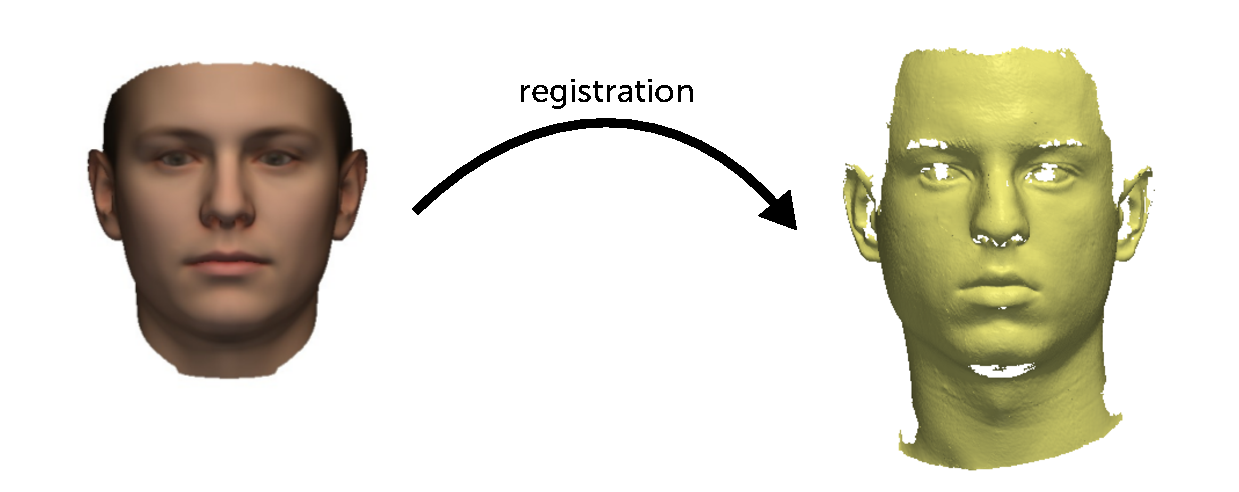
\includegraphics[width=\textwidth]{../resources/figures/intro1.pdf}
        \end{figure}
    \end{frame}

%%%%%%%%%%%%%%%%%%%%%%%%%%%%%%%%%%%%%%%%%%%%%%%%%%%%%%
    \begin{frame}{Registration Overview}
        \begin{figure}
            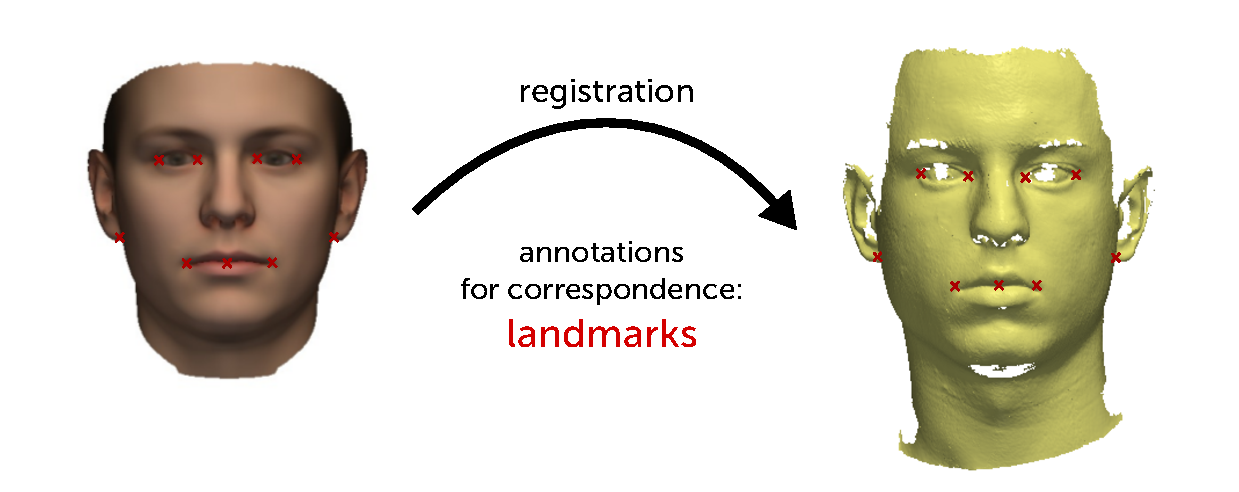
\includegraphics[width=\textwidth]{../resources/figures/intro2.pdf}
        \end{figure}
    \end{frame}

%%%%%%%%%%%%%%%%%%%%%%%%%%%%%%%%%%%%%%%%%%%%%%%%%%%%%%
    \begin{frame}{Registration Overview}
        \begin{figure}
            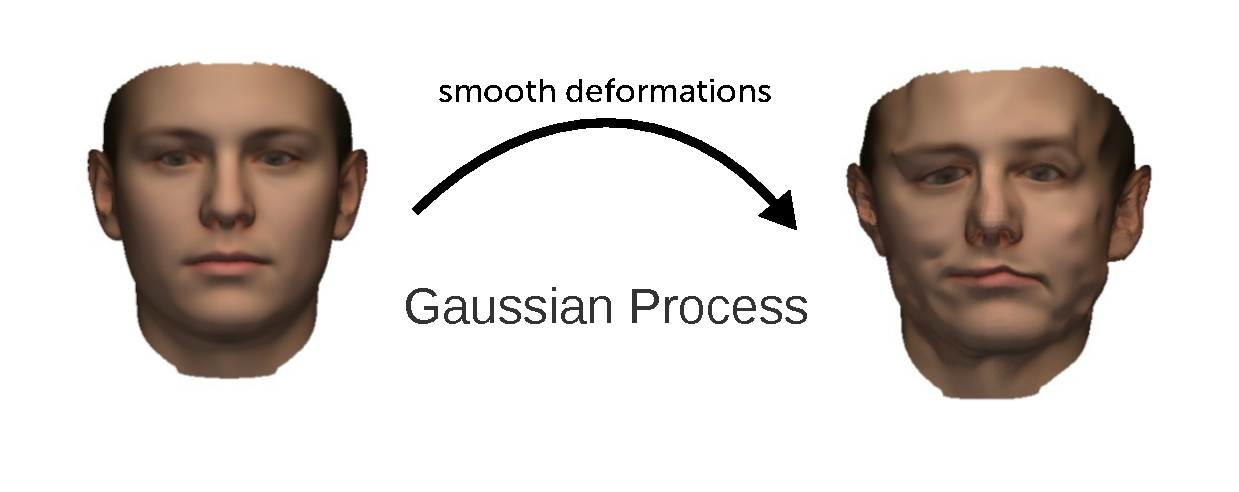
\includegraphics[width=\textwidth]{../resources/figures/intro3.pdf}
        \end{figure}
    \end{frame}

%%%%%%%%%%%%%%%%%%%%%%%%%%%%%%%%%%%%%%%%%%%%%%%%%%%%%%
    \begin{frame}{Registration Overview}
        \begin{figure}
            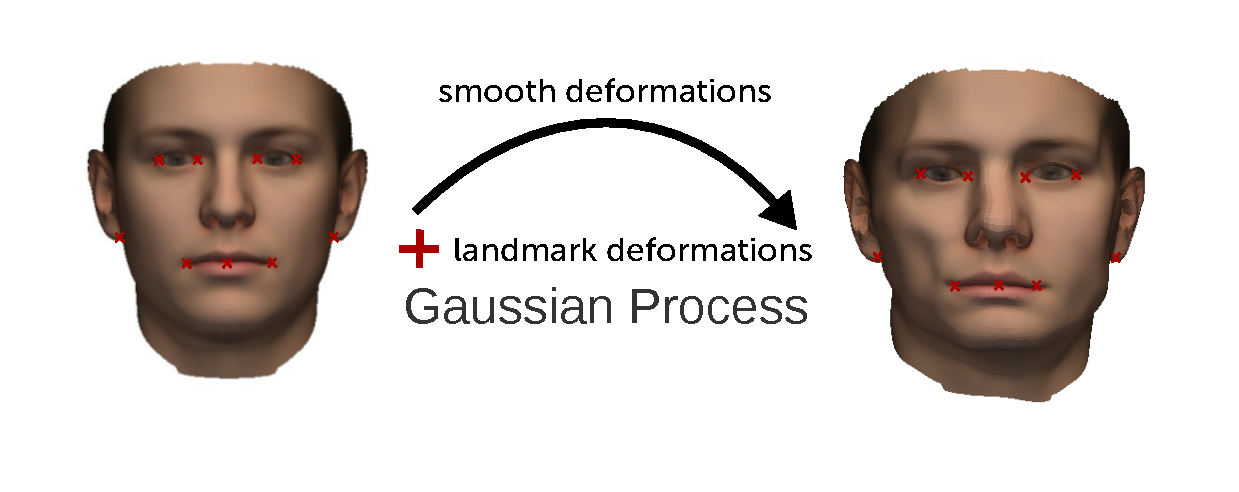
\includegraphics[width=\textwidth]{../resources/figures/intro4.pdf}
        \end{figure}
    \end{frame}


%%%%%%%%%%%%%%%%%%%%%%%%%%%%%%%%%%%%%%%%%%%%%%%%%%%%%%
    \begin{frame}{Registration Overview}
        \begin{figure}
            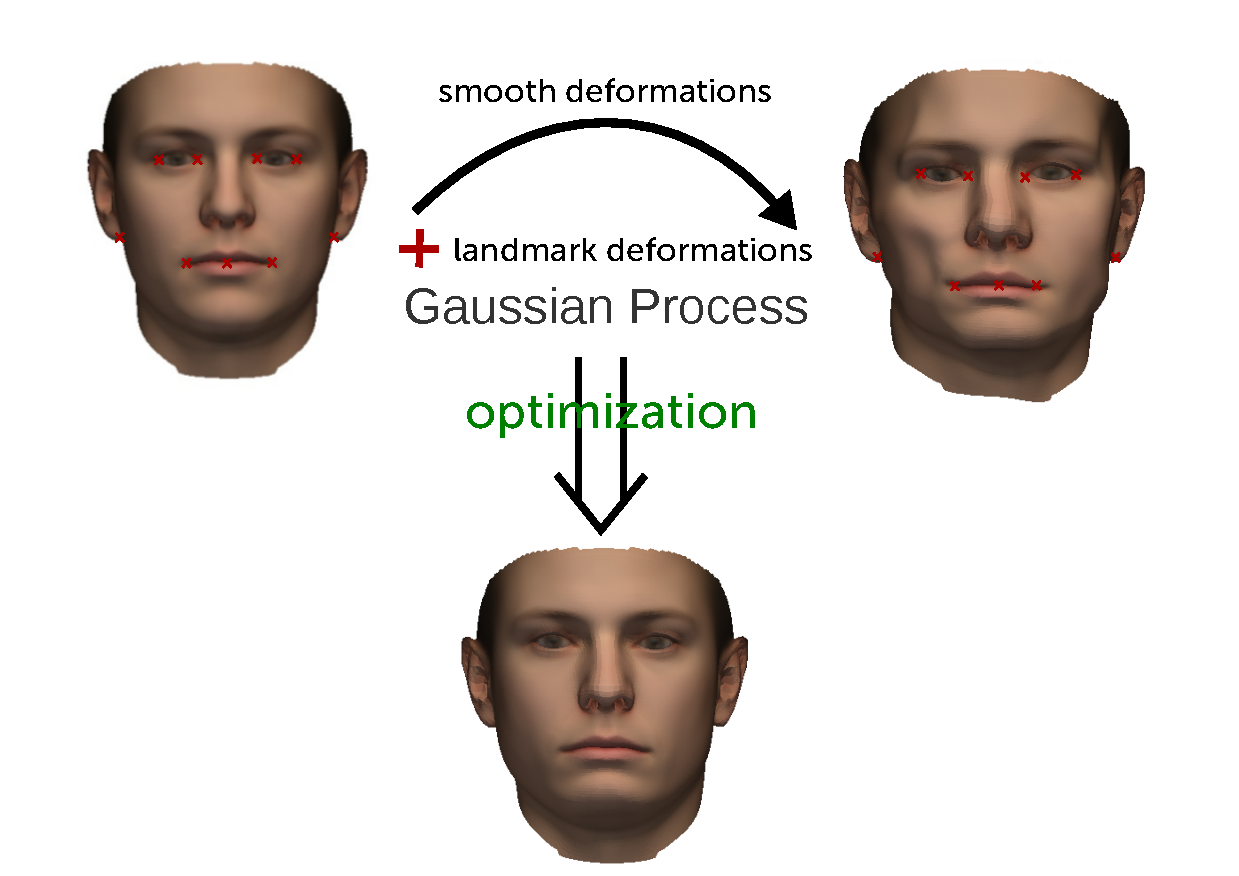
\includegraphics[width=\textwidth]{../resources/figures/intro5.pdf}
        \end{figure}
    \end{frame}

%%%%%%%%%%%%%%%%%%%%%%%%%%%%%%%%%%%%%%%%%%%%%%%%%%%%%%
    \begin{frame}{Registration Overview}
        \begin{figure}
            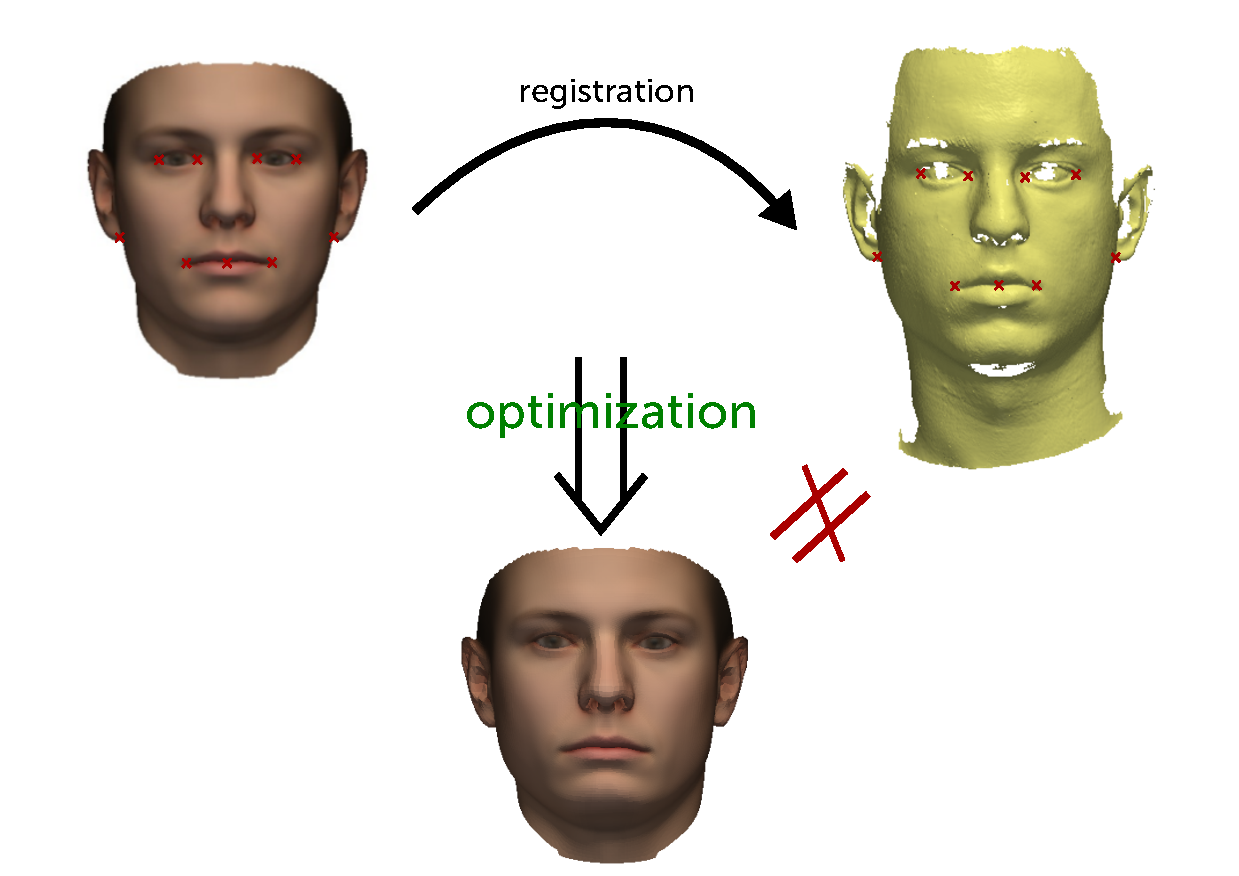
\includegraphics[width=\textwidth]{../resources/figures/intro6.pdf}
        \end{figure}
    \end{frame}

%%%%%%%%%%%%%%%%%%%%%%%%%%%%%%%%%%%%%%%%%%%%%%%%%%%%%%
    \begin{frame}{Registration Overview}
        \begin{figure}
            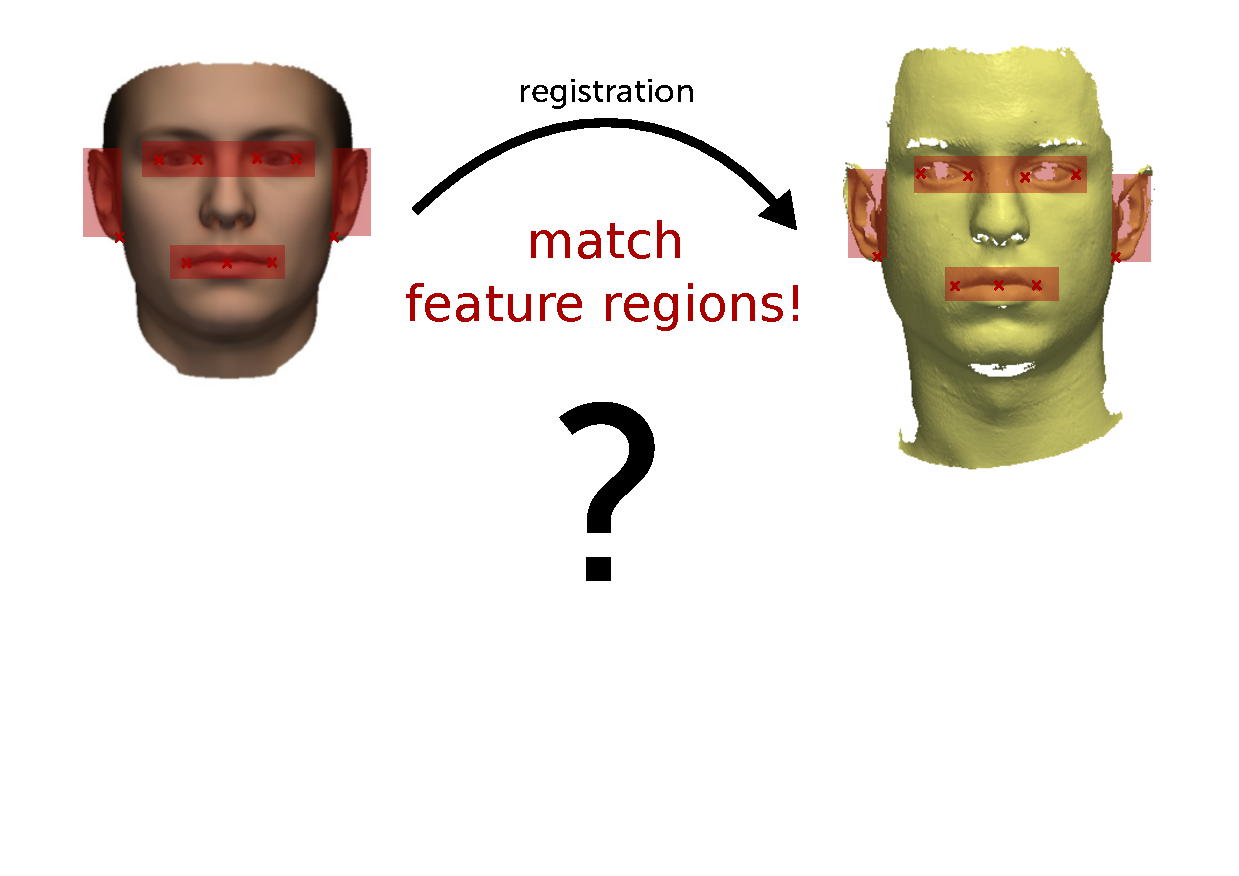
\includegraphics[width=\textwidth]{../resources/figures/intro7.pdf}
        \end{figure}
    \end{frame}

%%%%%%%%%%%%%%%%%%%%%%%%%%%%%%%%%%%%%%%%%%%%%%%%%%%%%%
    \begin{frame}{Pipeline}
        \begin{figure}
            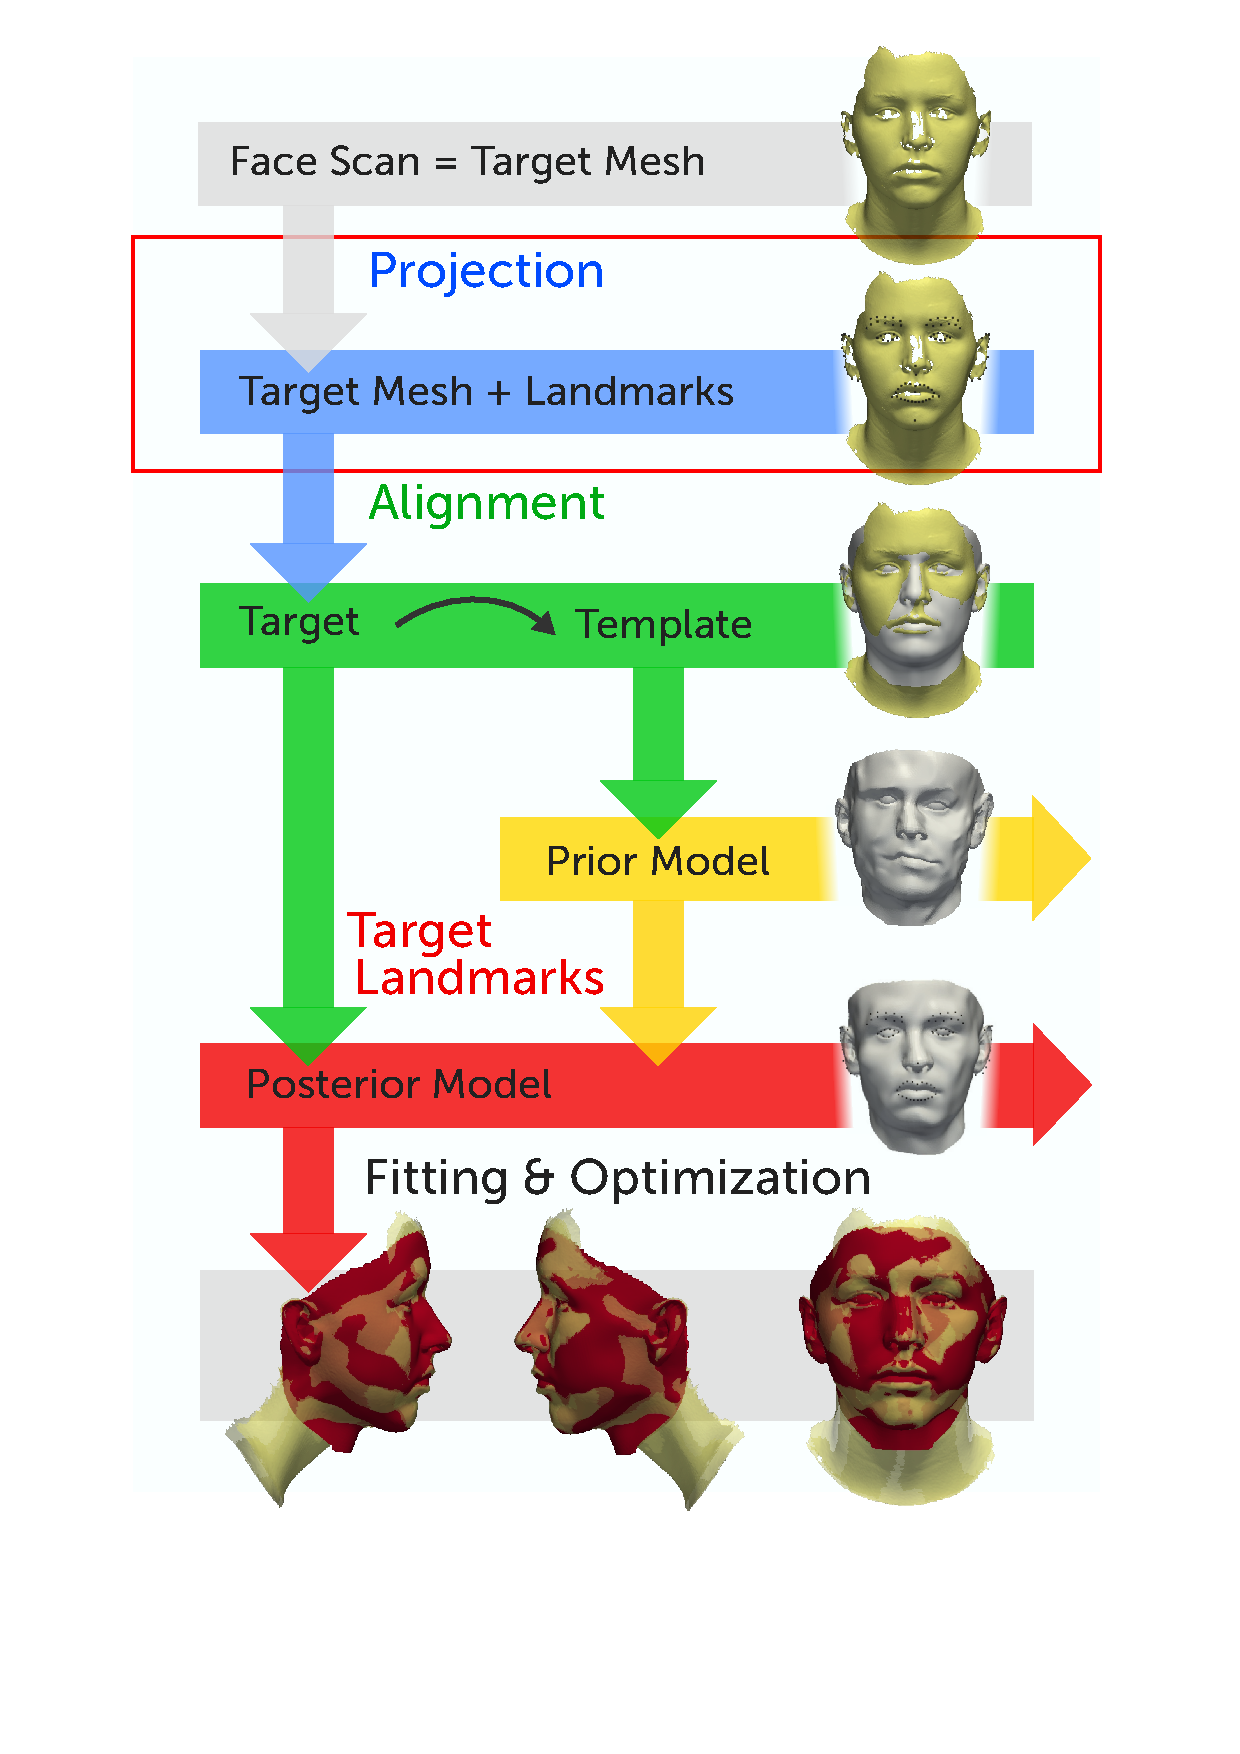
\includegraphics[width=.5\textwidth]{../resources/figures/pipeline_linefeature.pdf}
        \end{figure}
    \end{frame}

%%%%%%%%%%%%%%%%%%%%%%%%%%%%%%%%%%%%%%%%%%%%%%%%%%%%%%
%%%%%%%%%%%%%%%%%%%%%%%%%%%%%%%%%%%%%%%%%%%%%%%%%%%%%%
    \section{\scshape Data and Correspondence}
    \begin{frame}{Data and Correspondence}
        \begin{figure}
            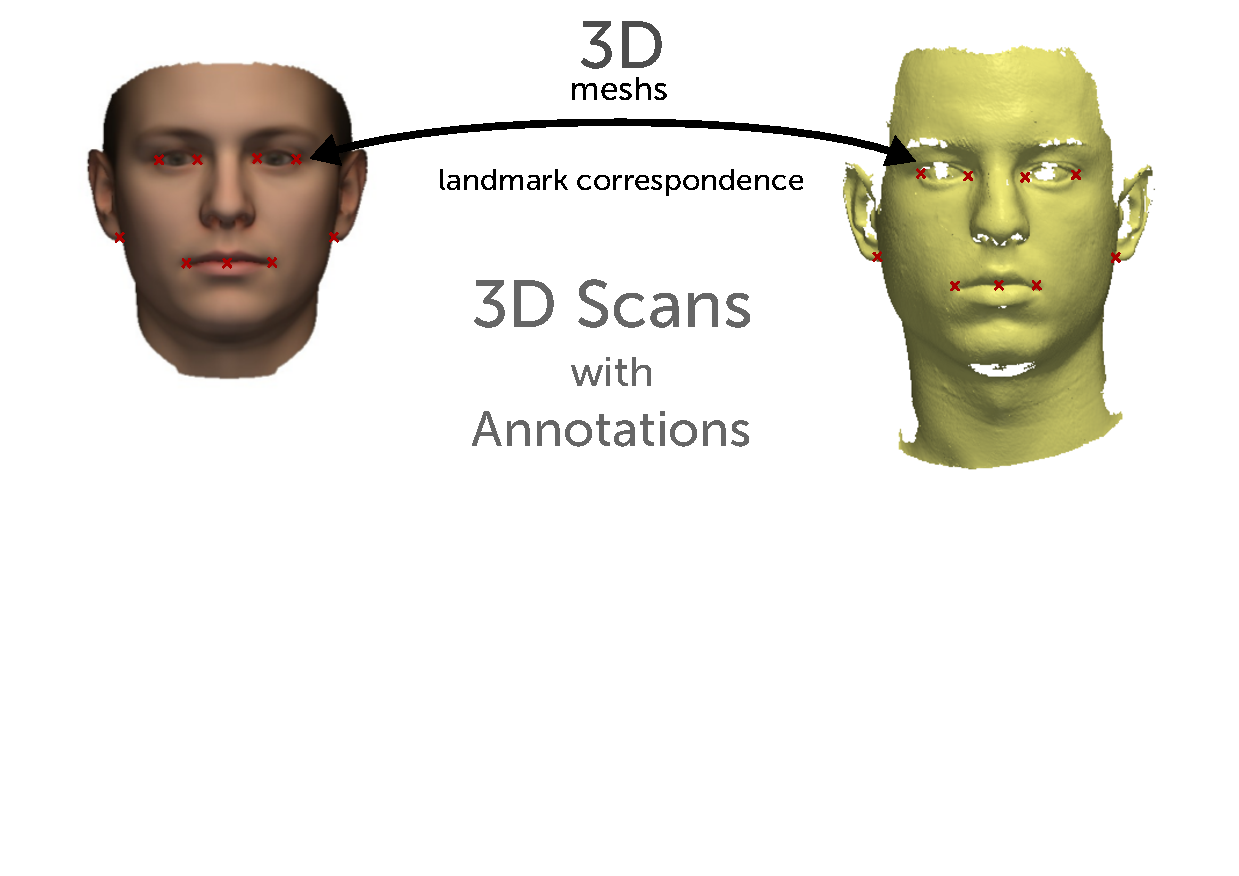
\includegraphics[width=.9\textwidth]{../resources/figures/givendata1.pdf}
        \end{figure}
    \end{frame}

%%%%%%%%%%%%%%%%%%%%%%%%%%%%%%%%%%%%%%%%%%%%%%%%%%%%%%
    \begin{frame}{Data and Correspondence}
        \begin{figure}
            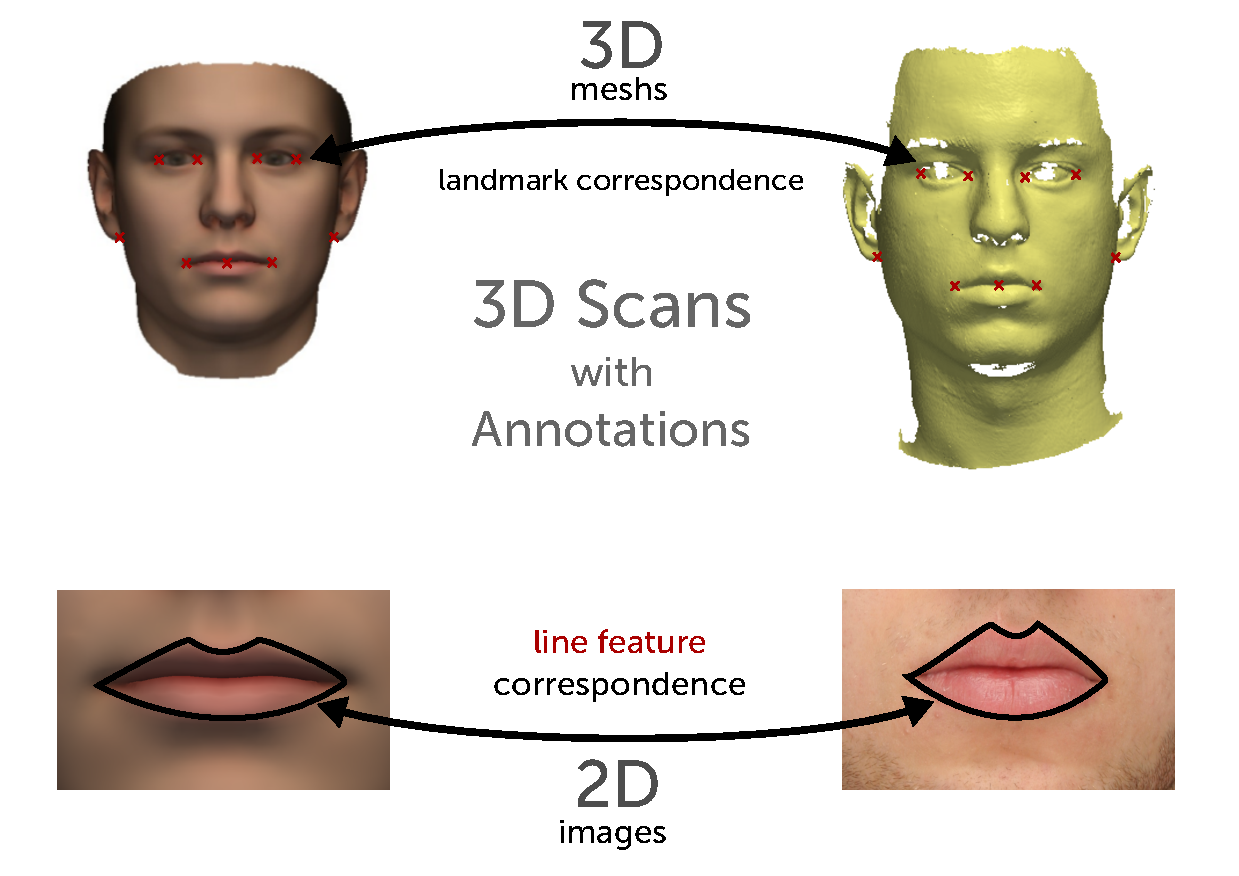
\includegraphics[width=.9\textwidth]{../resources/figures/givendata2.pdf}
        \end{figure}
    \end{frame}

%%%%%%%%%%%%%%%%%%%%%%%%%%%%%%%%%%%%%%%%%%%%%%%%%%%%%%
    \begin{frame}{Data and Correspondence}
        \begin{figure}
            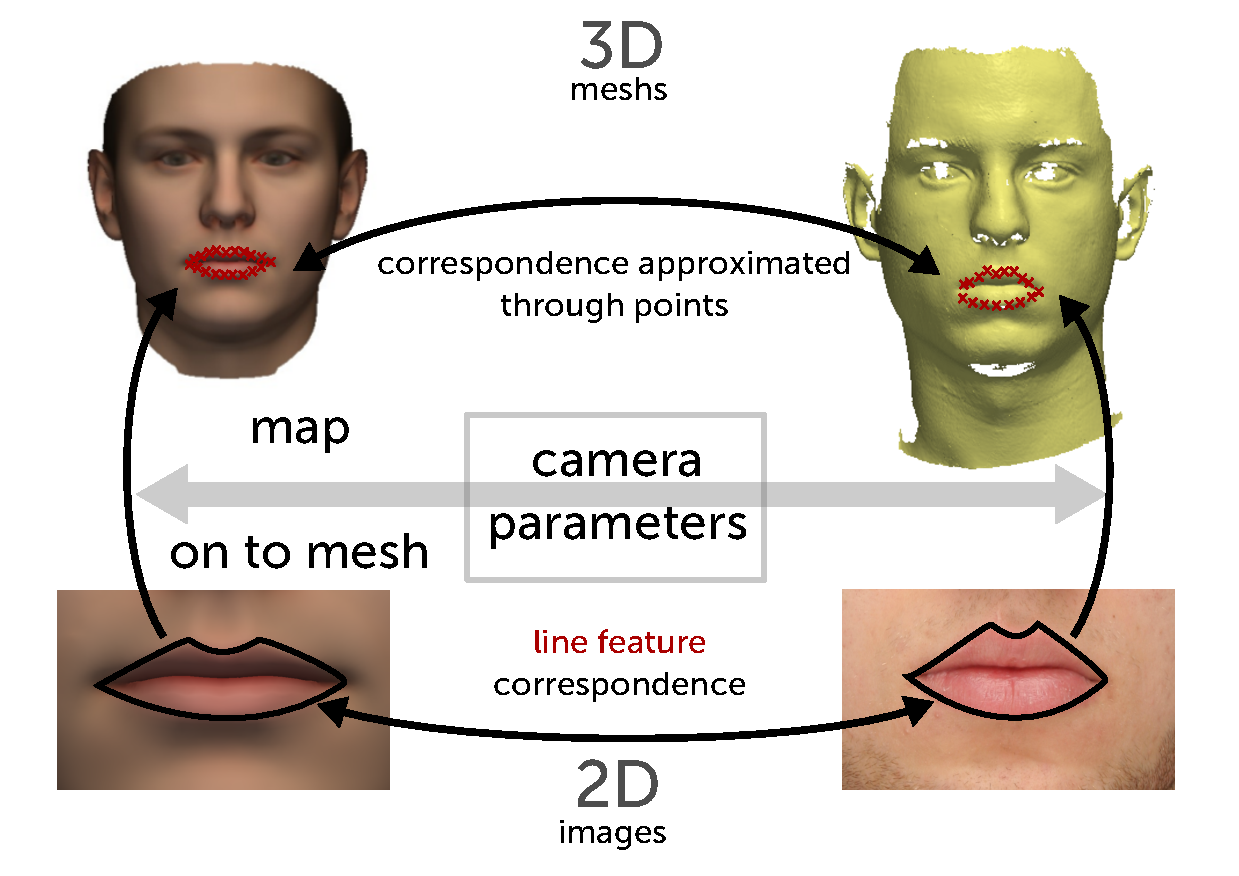
\includegraphics[width=.9\textwidth]{../resources/figures/givendata3.pdf}
        \end{figure}
    \end{frame}

%%%%%%%%%%%%%%%%%%%%%%%%%%%%%%%%%%%%%%%%%%%%%%%%%%%%%%
    \section{\scshape Using Line Features}
    \subsection{Sampling Line Features}
%%%%%%%%%%%%%%%%%%%%%%%%%%%%%%%%%%%%%%%%%%%%%%%%%%%%%%
    \begin{frame}{Mapping Line Features}
        Idea: Sample points from the line features and use them as additional landmarks
        \begin{figure}
            \centering
            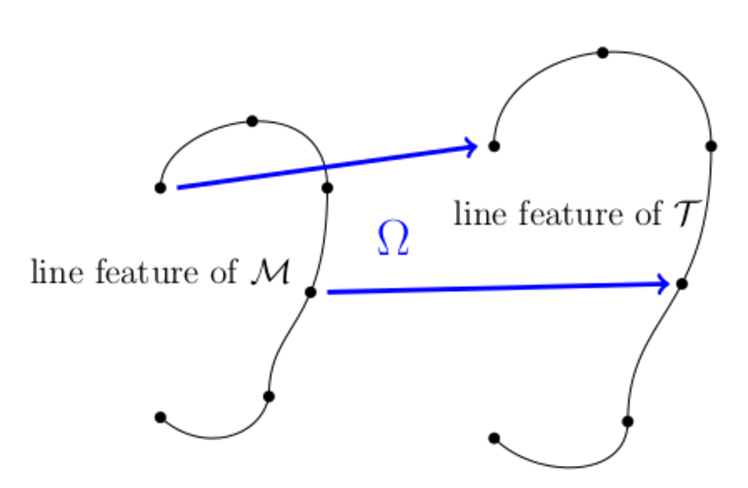
\includegraphics[width=.5\textwidth]{../resources/img/linefeaturemapping.pdf}
        \end{figure}
        \textit{What about correspondence?}
    \end{frame}

%%%%%%%%%%%%%%%%%%%%%%%%%%%%%%%%%%%%%%%%%%%%%%%%%%%%%%
    \begin{frame}{Equidistant Sampling}
        Approximate correspondance by sampling line features in equidistant intervals
        \begin{figure}
            \centering
            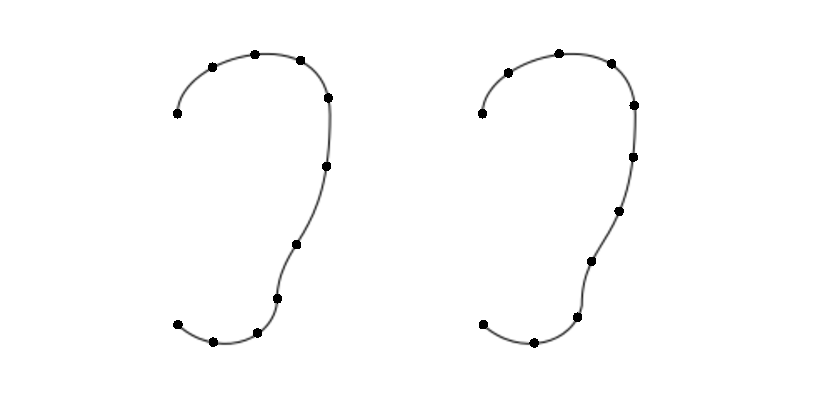
\includegraphics[width=.7\textwidth]{../resources/figures/ears_diffparam.pdf}
        \end{figure}
    \end{frame}

%%%%%%%%%%%%%%%%%%%%%%%%%%%%%%%%%%%%%%%%%%%%%%%%%%%%%%
    \begin{frame}{B\'{e}zier curves}
        Line features consist of B\'{e}zier curve segments\\
        $\rightarrow$ underlying parameter is not linear\\
        \bigskip
        Approximate arc-length of curve through euclidean distance of sampled points\\
        \begin{figure}
            \centering
            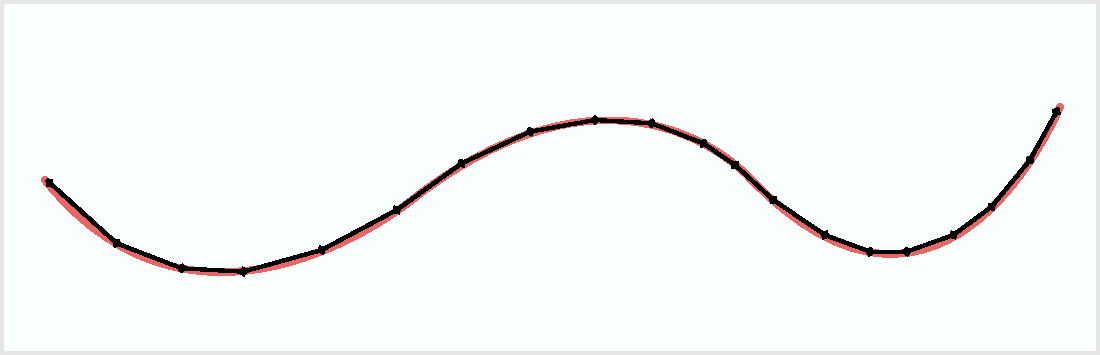
\includegraphics[width=.7\textwidth]{../resources/figures/distance_computation.pdf}
        \end{figure}
        $\Rightarrow$ map point coordinates to approximated fractional length of curve
    \end{frame}

%%%%%%%%%%%%%%%%%%%%%%%%%%%%%%%%%%%%%%%%%%%%%%%%%%%%%%
    \subsection{Projection: 2D to 3D}
    \begin{frame}{Pipeline: Projection}
        \begin{figure}   
            \centering
            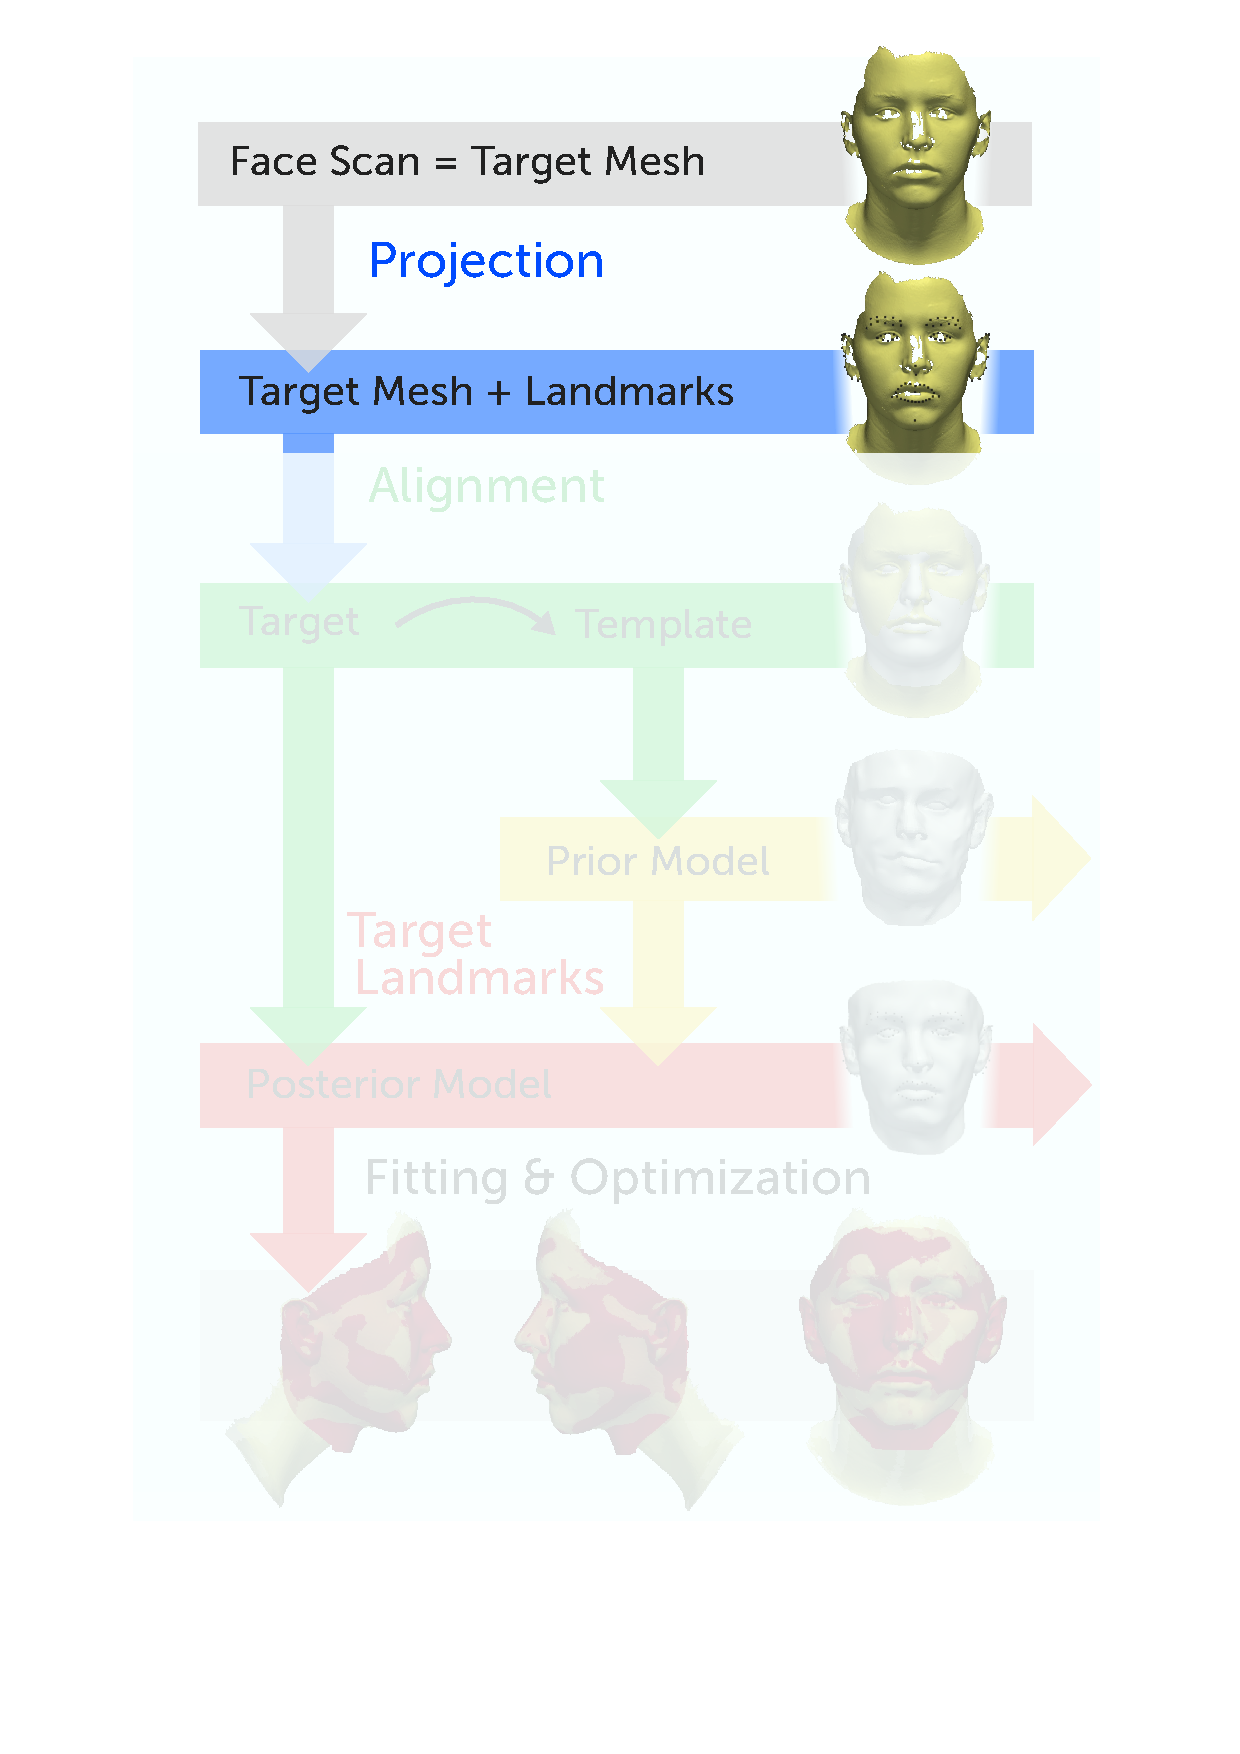
\includegraphics[width=.6\textwidth]{../resources/figures/pipeline_projection.pdf}
        \end{figure}
    \end{frame}

    \begin{frame}{Projection: 2D to 3D}
        \begin{figure}
            \centering
            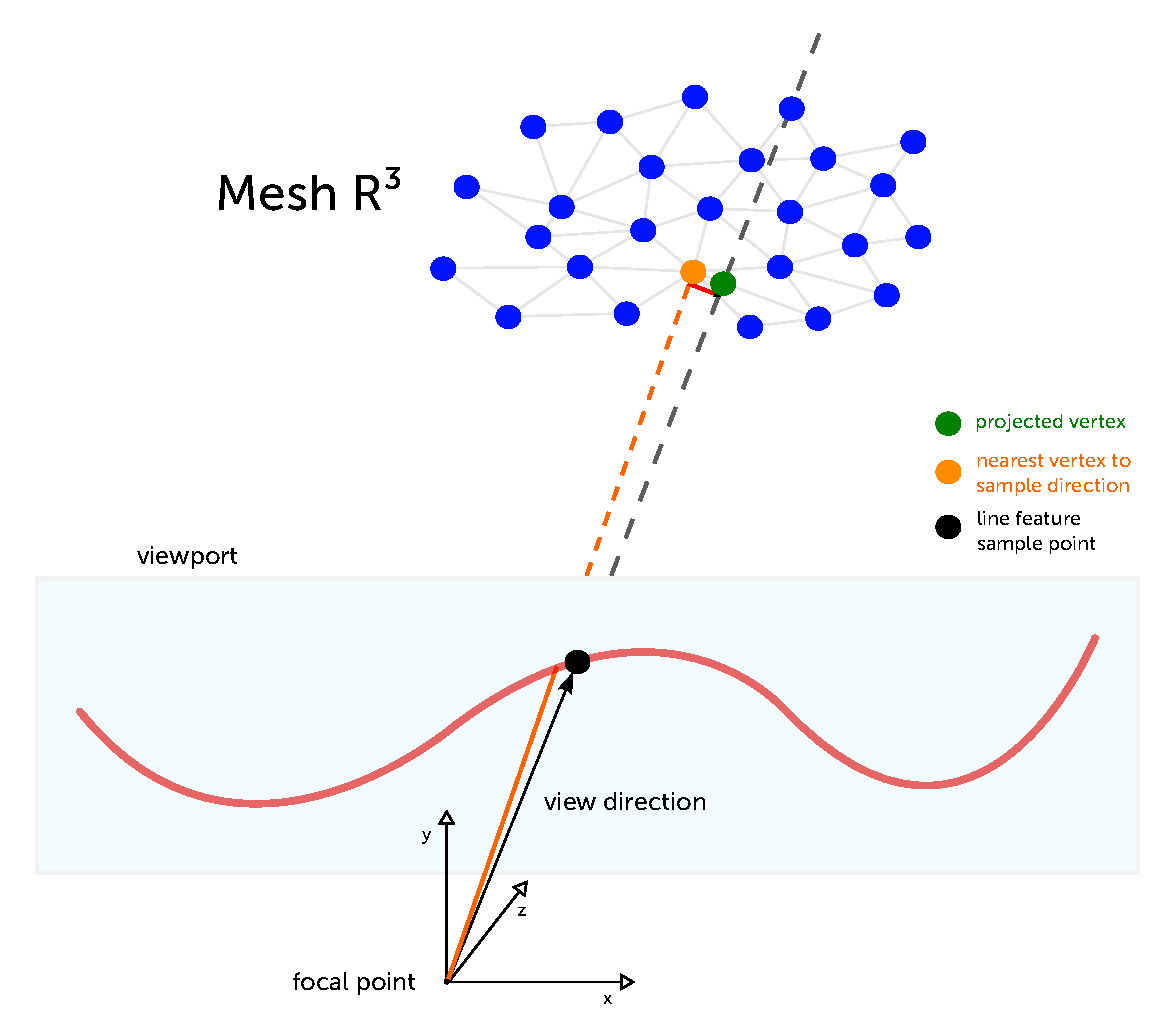
\includegraphics[width=.8\textwidth]{../resources/figures/projection.pdf}
        \end{figure}
    \end{frame}

    \begin{frame}{Target Mesh Holes}
        \begin{figure}
            \centering
            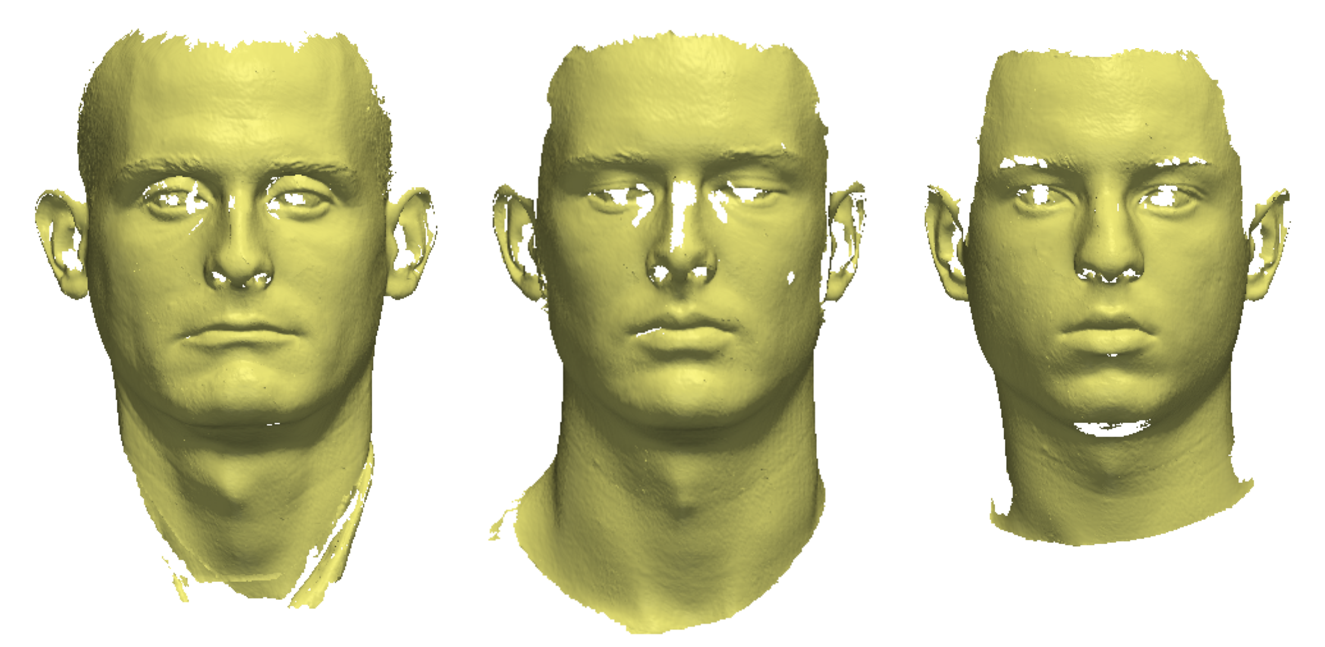
\includegraphics[width=.8\textwidth]{../resources/img/holes.pdf}
        \end{figure}
    \end{frame}

    \begin{frame}{Projection: holes}
        \begin{figure}
            \centering
            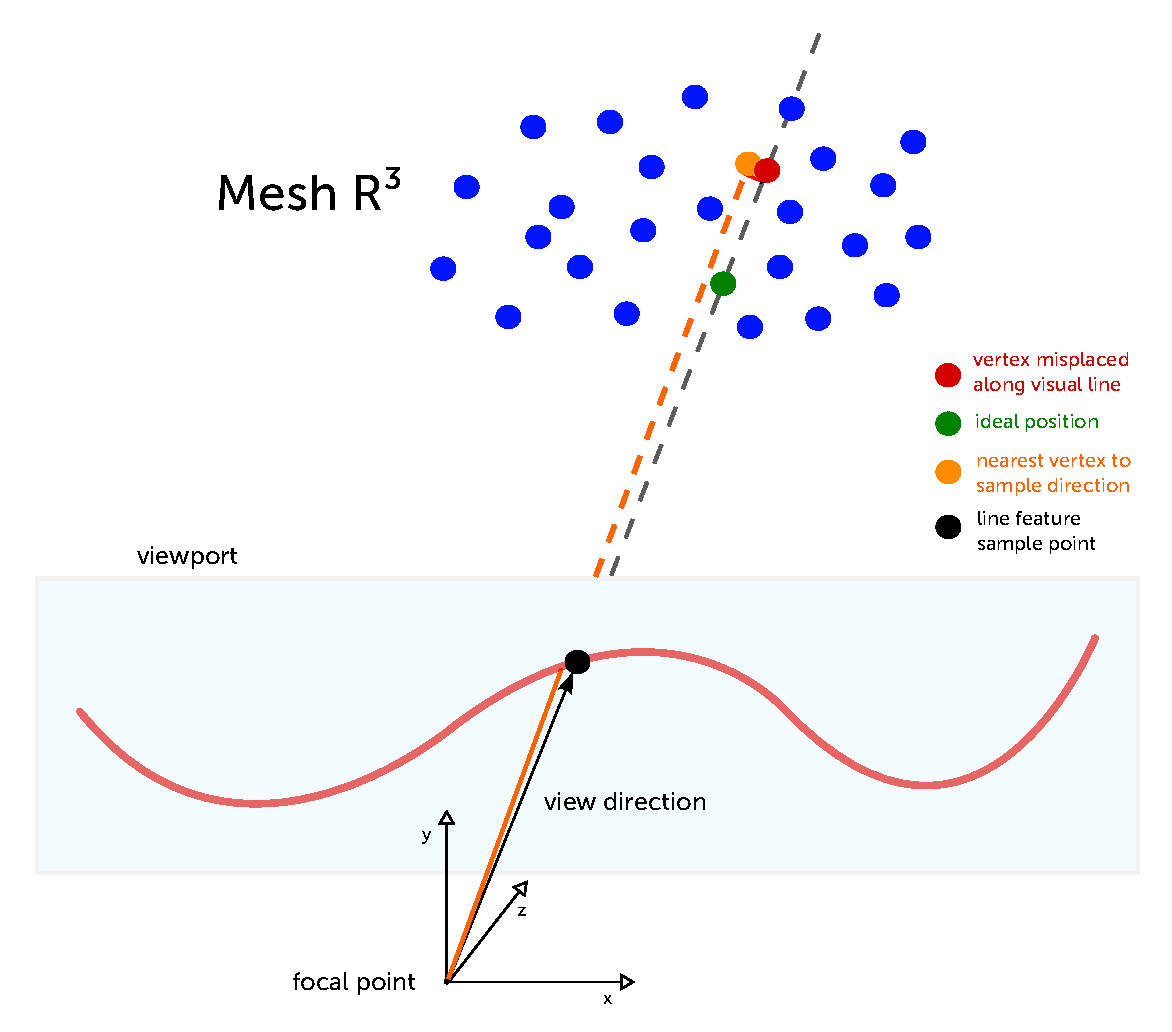
\includegraphics[width=.8\textwidth]{../resources/figures/projection_holes.pdf}
        \end{figure}
    \end{frame}


    \subsection{Results of 3D representation}
    \begin{frame}{3D representation}
         \begin{figure}
            \centering
            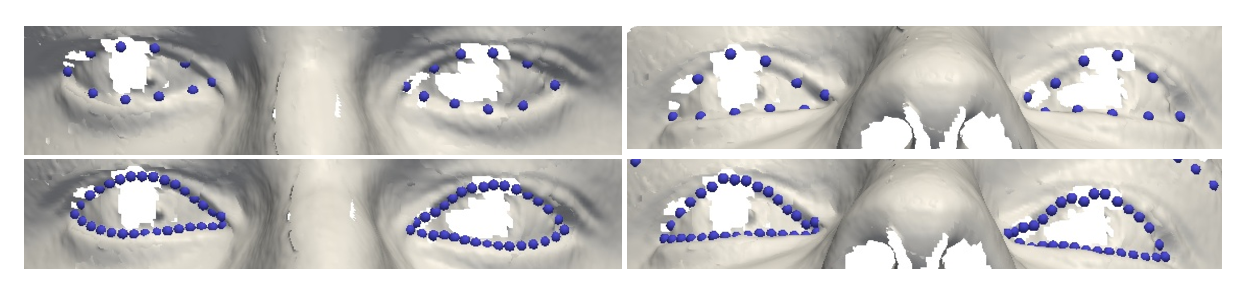
\includegraphics[width=\textwidth]{../resources/img/linefeatures_eyes.pdf}
        \end{figure}
    \end{frame}

    \begin{frame}{Template/Target Alignment}
        \begin{figure}   
            \centering
            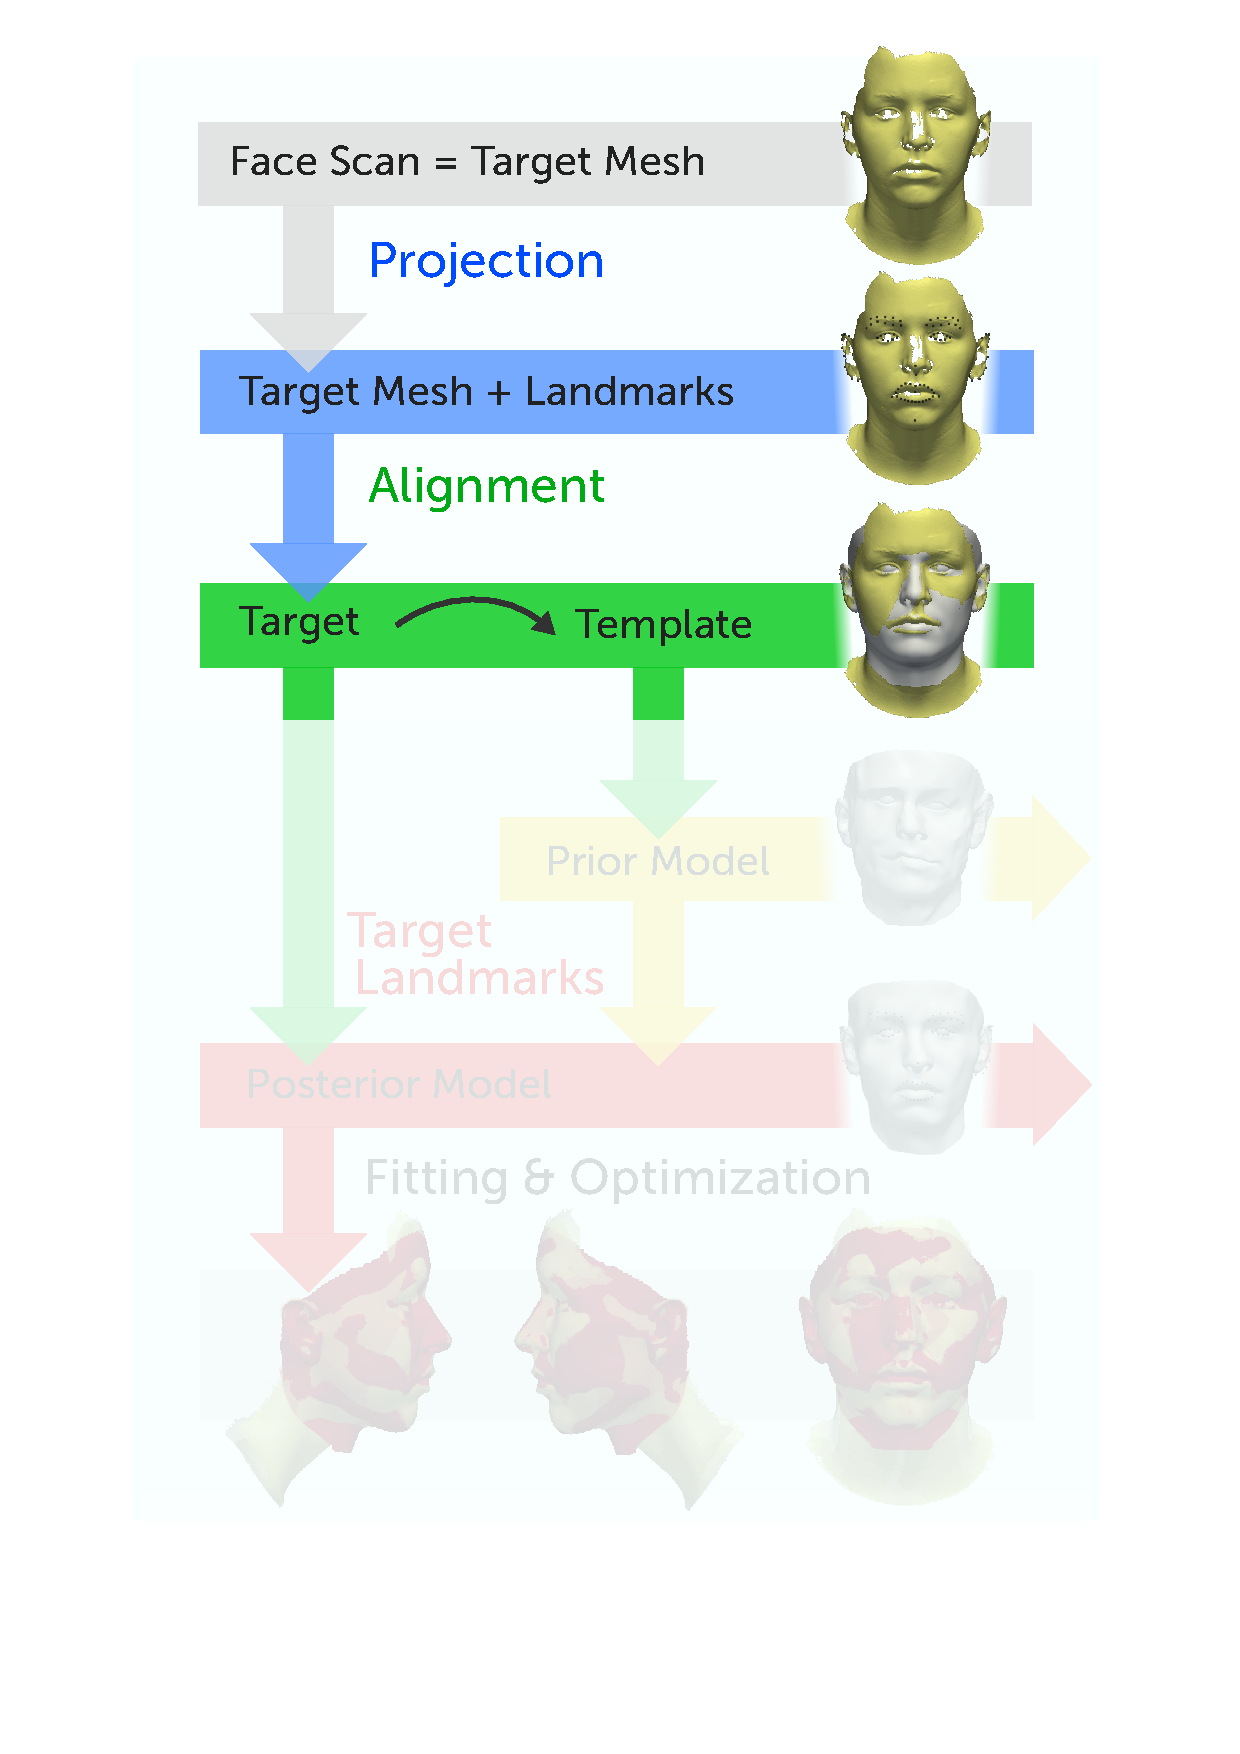
\includegraphics[width=.6\textwidth]{../resources/figures/pipeline_alignment.pdf}
        \end{figure}
    \end{frame}

    \begin{frame}{Template/Target Alignment}
        \begin{figure}   
            \centering
            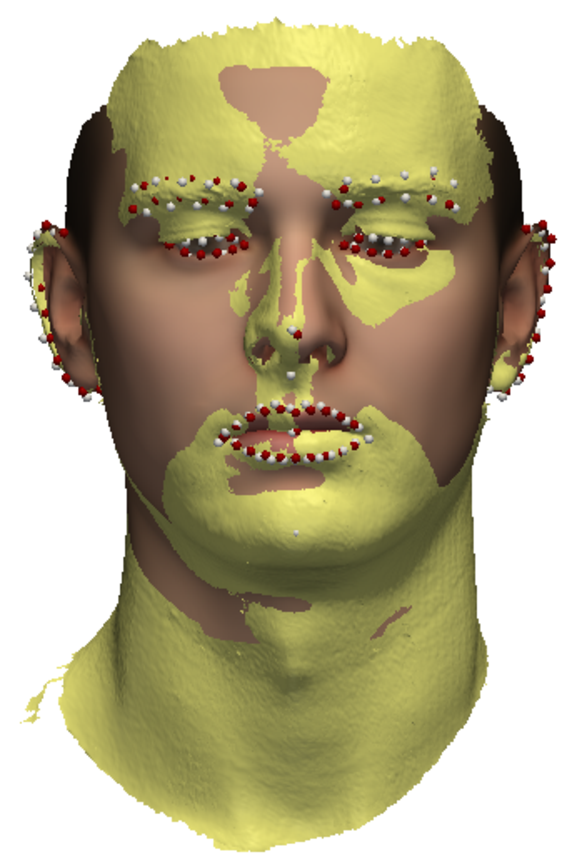
\includegraphics[width=.6\textwidth]{../resources/img/alignment.pdf}
        \end{figure}
    \end{frame}

%%%%%%%%%%%%%%%%%%%%%%%%%%%%%%%%%%%%%%%%%%%%%%%%%%%%%%
%%%%%%%%%%%%%%%%%%%%%%%%%%%%%%%%%%%%%%%%%%%%%%%%%%%%%%
    \section{\scshape Gaussian Process Regression}
    \subsection{Gaussian Process}
    \begin{frame}{Gaussian Process}
        intuitive: a generalization of the normal distribution to functions\\
        \bigskip
        a stochastic process where each random variable represents possible function values at a specific input point
    \end{frame}

%%%%%%%%%%%%%%%%%%%%%%%%%%%%%%%%%%%%%%%%%%%%%%%%%%%%%%
    \subsection{GP Prior}
    \begin{frame}{GP Prior}
        sample functions from the space of possible inputs\\
        these functions are defined by the covariance of the input points\\
        \begin{figure}
            \centering
            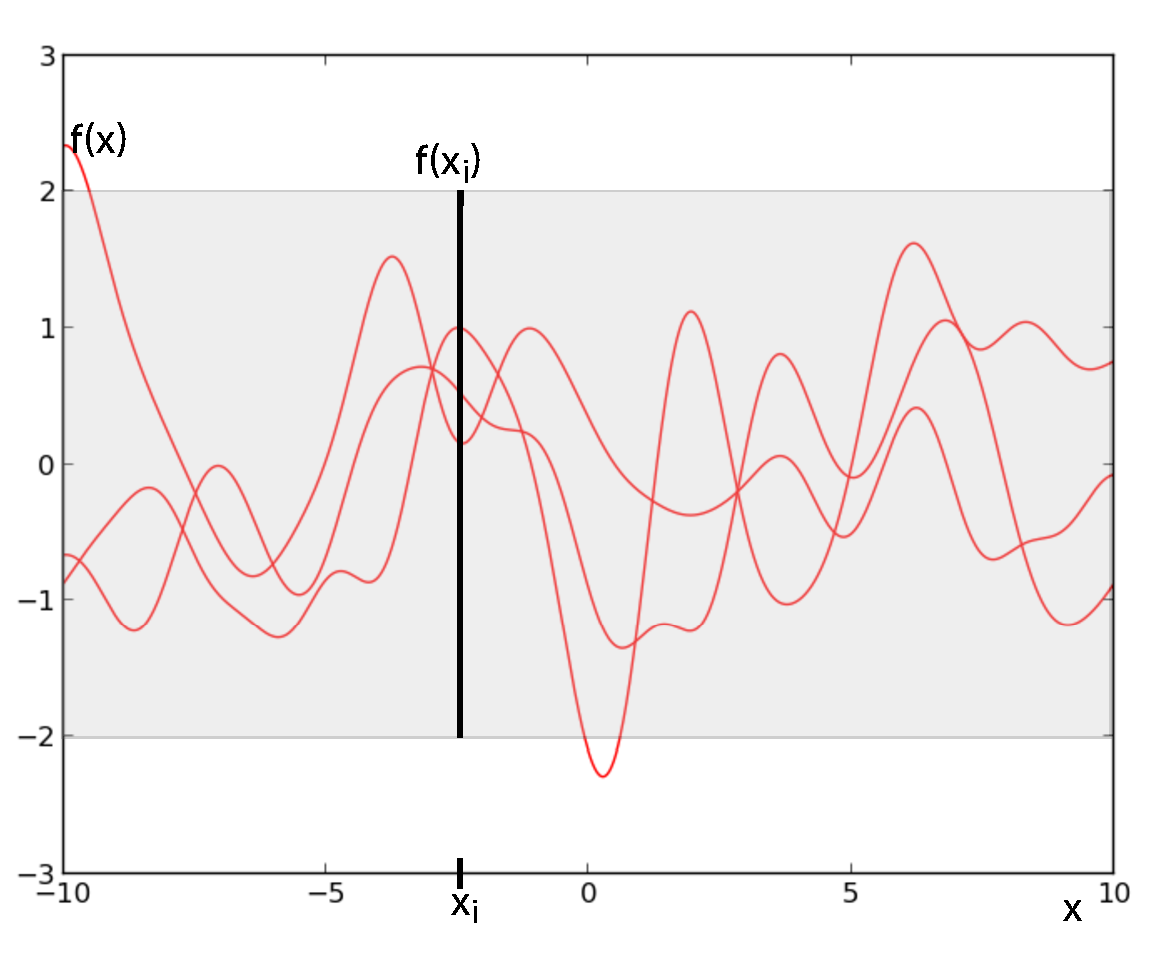
\includegraphics[width=.6\textwidth]{../resources/figures/gp_prior_new.pdf}
            \caption{normal distribution over 1000 input points}
        \end{figure}

    \end{frame}

%%%%%%%%%%%%%%%%%%%%%%%%%%%%%%%%%%%%%%%%%%%%%%%%%%%%%%
    \subsection{GP Posterior}
    \begin{frame}{GP Posterior Distribution}
\begin{figure}
\centering
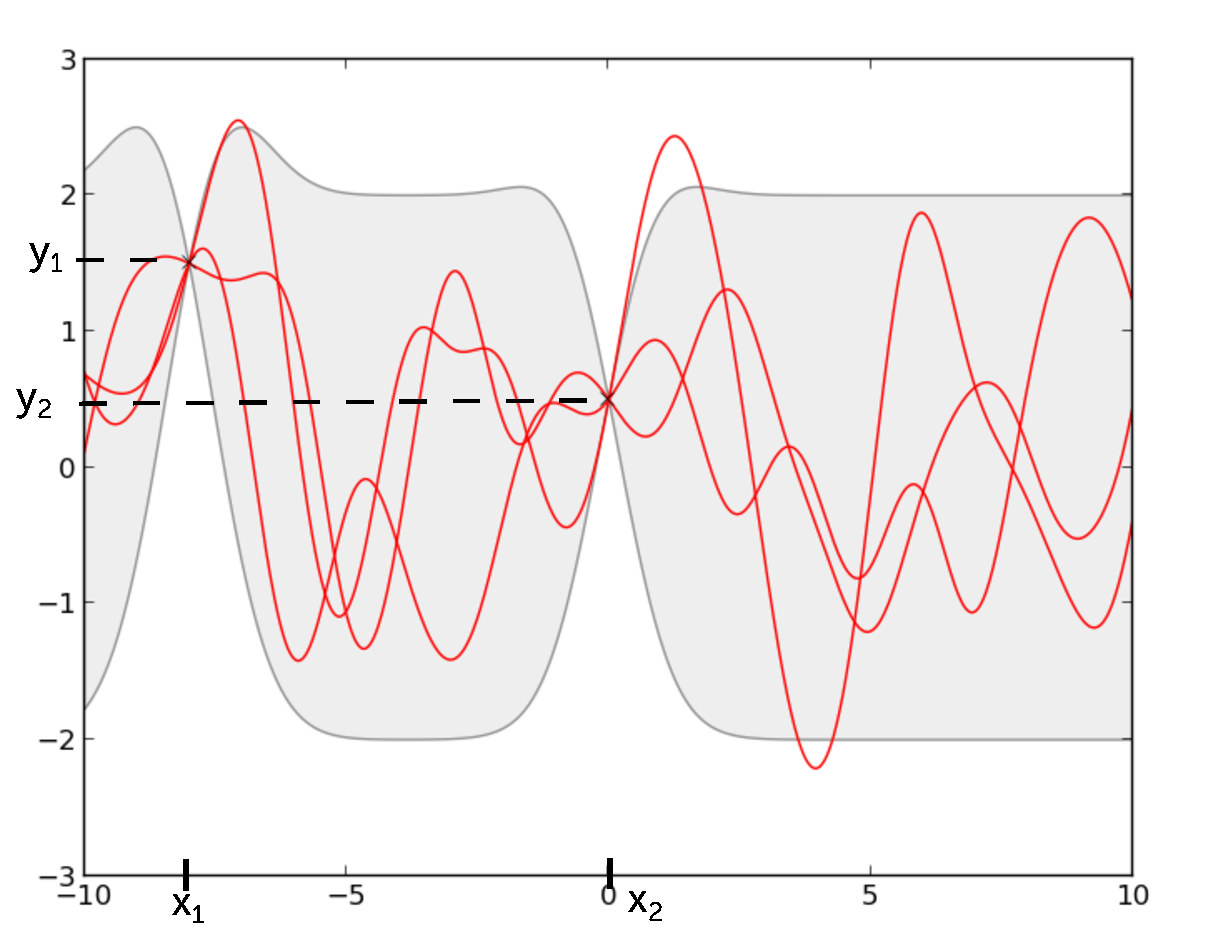
\includegraphics[width=.6\textwidth]{../resources/figures/gp_posterior_2.pdf}
\caption{posterior distribution fixed at 2 input points}
\end{figure}
    \end{frame}

\begin{frame}{GP Posterior Distribution}
\begin{figure}
\centering
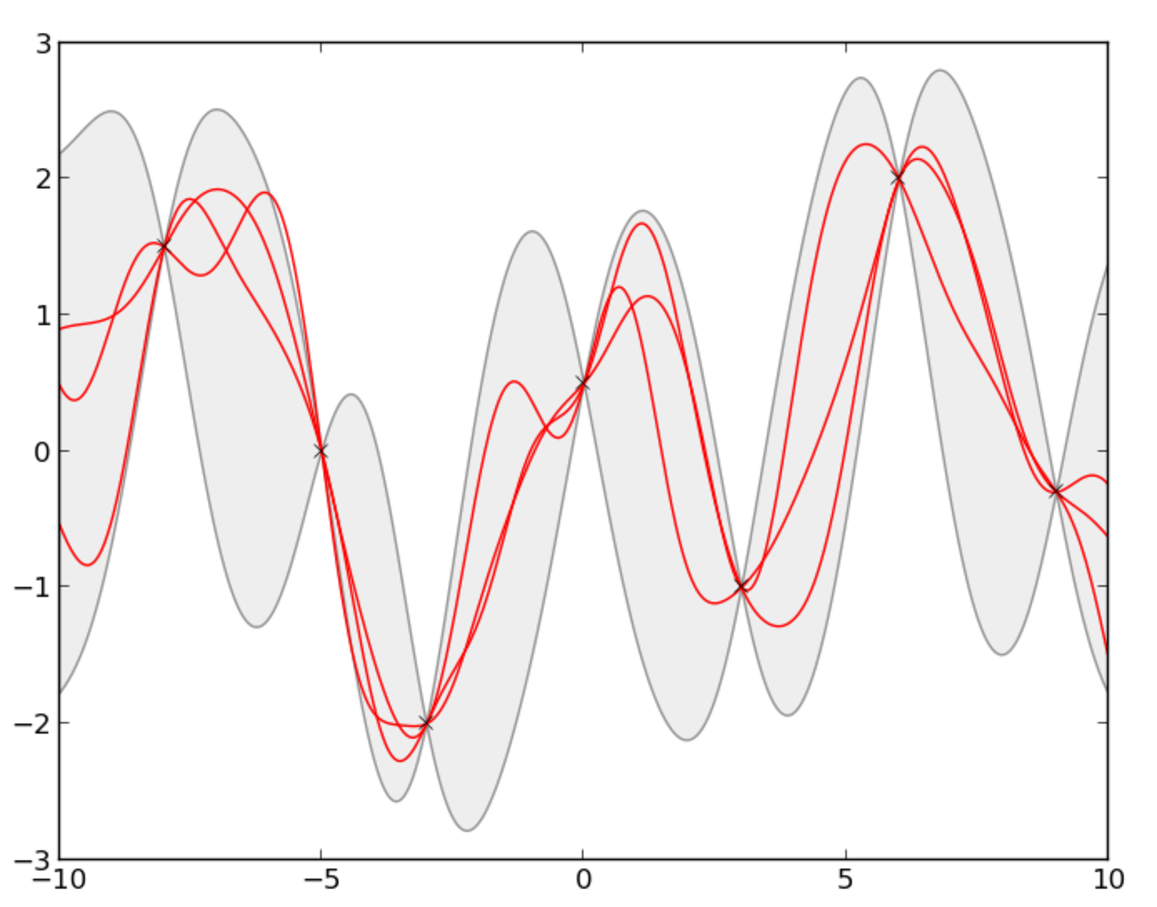
\includegraphics[width=.6\textwidth]{../resources/figures/gp_posterior.pdf}
\caption{posterior distribution fixed at 7 input points}
\end{figure}
\end{frame}

%%%%%%%%%%%%%%%%%%%%%%%%%%%%%%%%%%%%%%%%%%%%%%%%%%%%%%
%%%%%%%%%%%%%%%%%%%%%%%%%%%%%%%%%%%%%%%%%%%%%%%%%%%%%%
\subsection{Application to 3D Face Registration}
\begin{frame}{GPR in 3D Face Registration}
definition of Vector-valued GP
\begin{align*}
    & \mu: \mathcal{M} \rightarrow 0\\
    & k: \mathcal{M} \times \mathcal{M} \rightarrow \mathbb{R}^3 \times \mathbb{R}^3
\end{align*}
 \begin{figure}
        \centering
        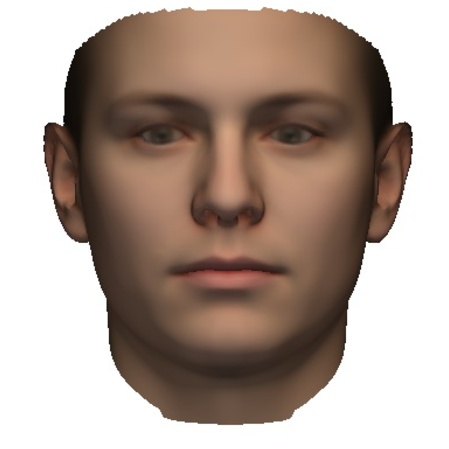
\includegraphics[width=.4\textwidth]{../resources/img/mean_msh.pdf}
    \end{figure}
\end{frame}

\begin{frame}{Pipeline: Deformation Prior}
\begin{figure}   
\centering
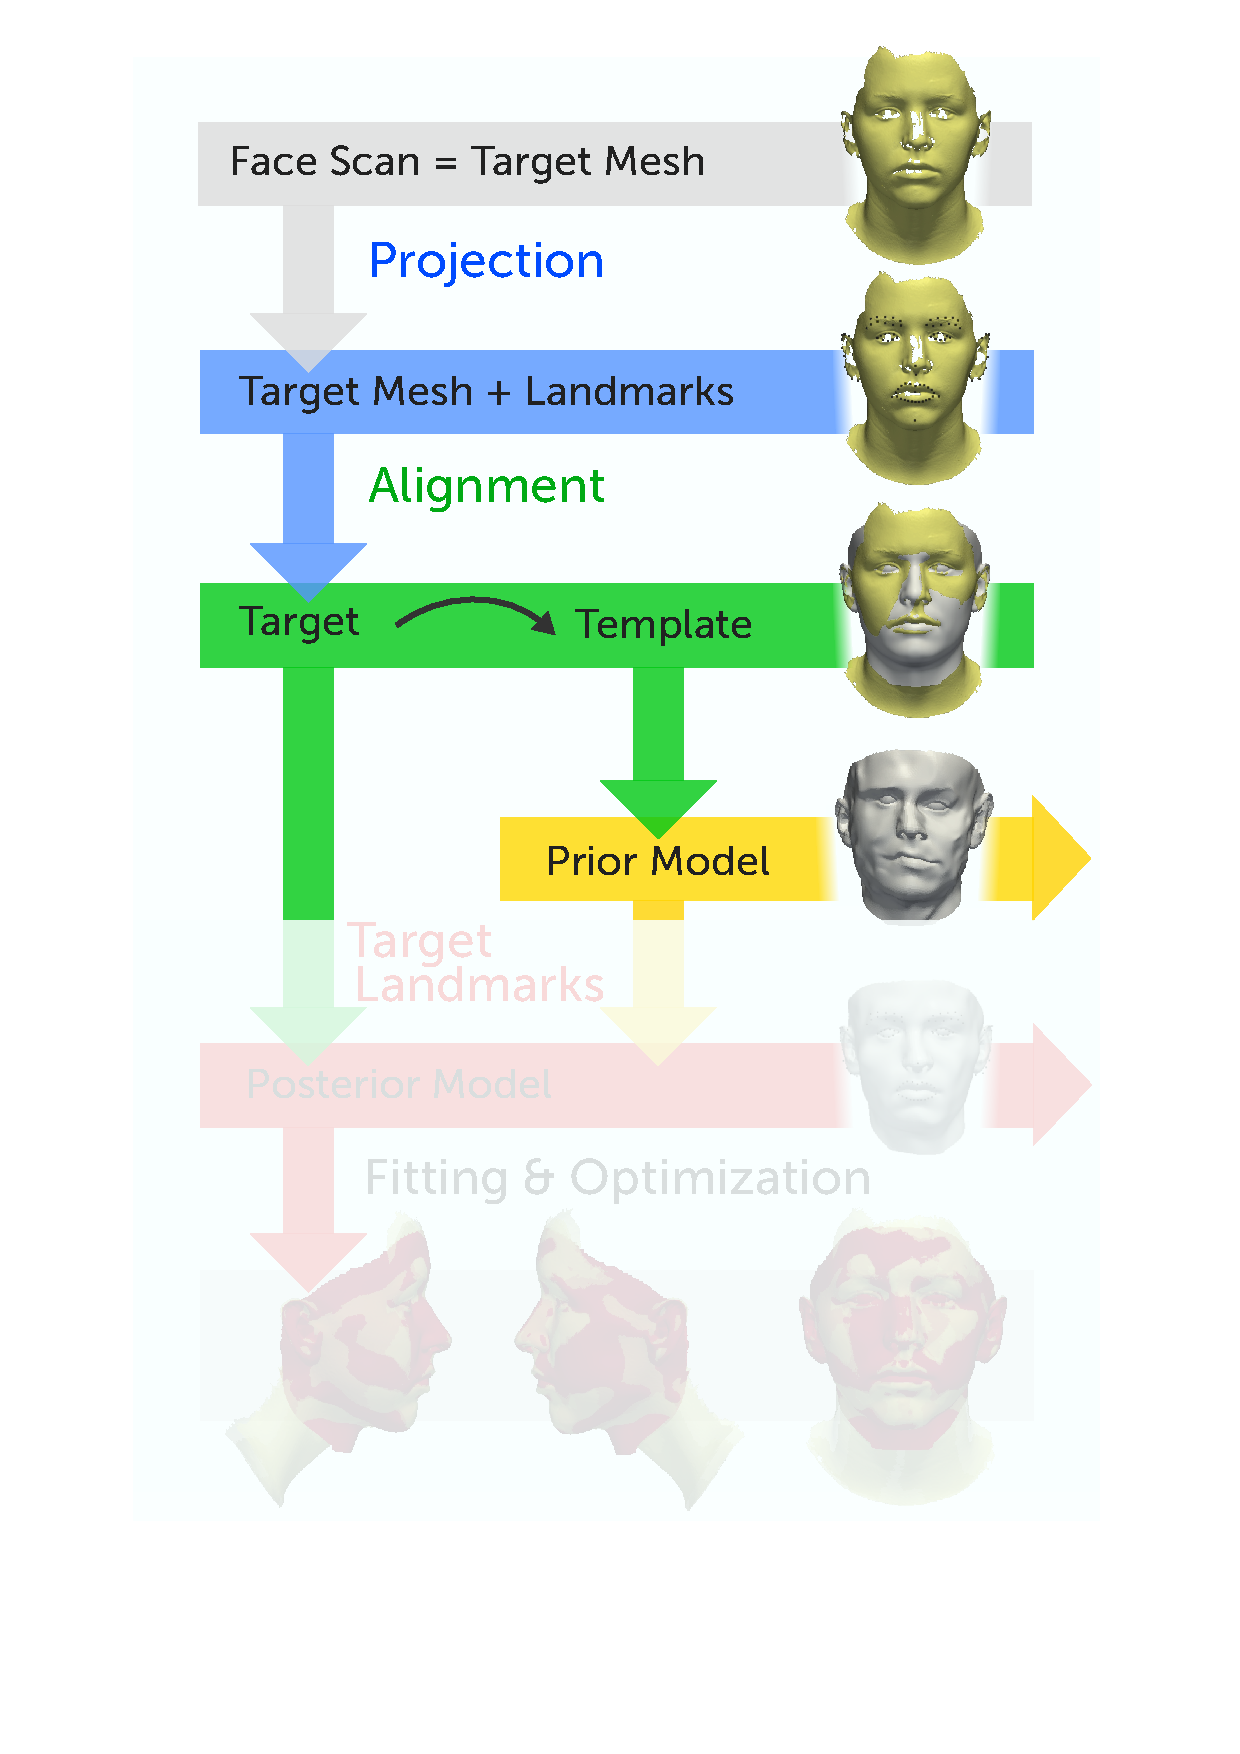
\includegraphics[width=.6\textwidth]{../resources/figures/pipeline_prior.pdf}
\end{figure}
%\begin{comment}
%projected line features on to face scans and template/mean mesh, now we want to define a prior distribution on the template mesh
%\end{comment}
\end{frame}

%%%%%%%%%%%%%%%%%%%%%%%%%%%%%%%%%%%%%%%%%%%%%%%%%%%%%%
\begin{frame}{Deformation Prior}
build GP Prior from template mesh vertices\\
\bigskip
$\Rightarrow$ GP defines a distribution of possible deformations of the template mesh 
\begin{figure}
    \centering
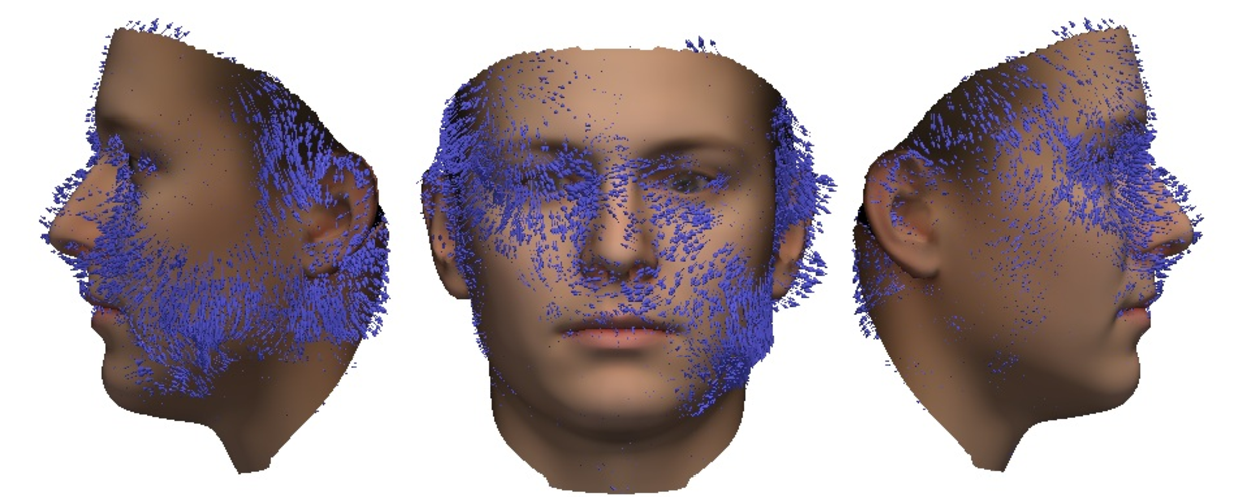
\includegraphics[width=.8\textwidth]{../resources/img/prior_deformations.pdf}
\end{figure}
\end{frame}

\begin{frame}{Prior faces}
    \begin{figure}
    \centering
    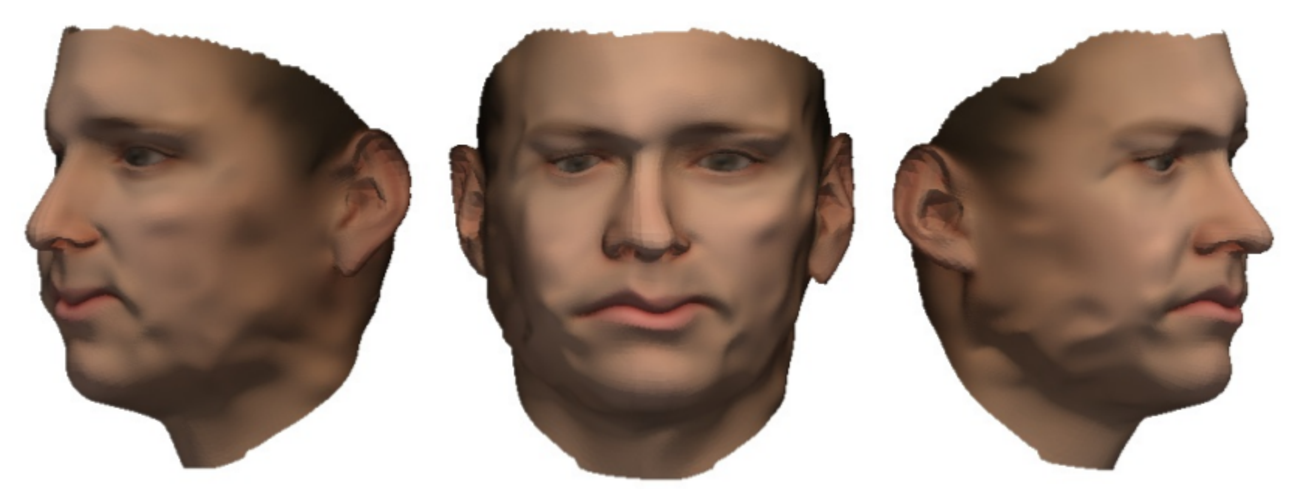
\includegraphics[width=.9\textwidth]{../resources/img/prior_sample_2_profile.pdf}
\end{figure}
\begin{figure}
    \centering
    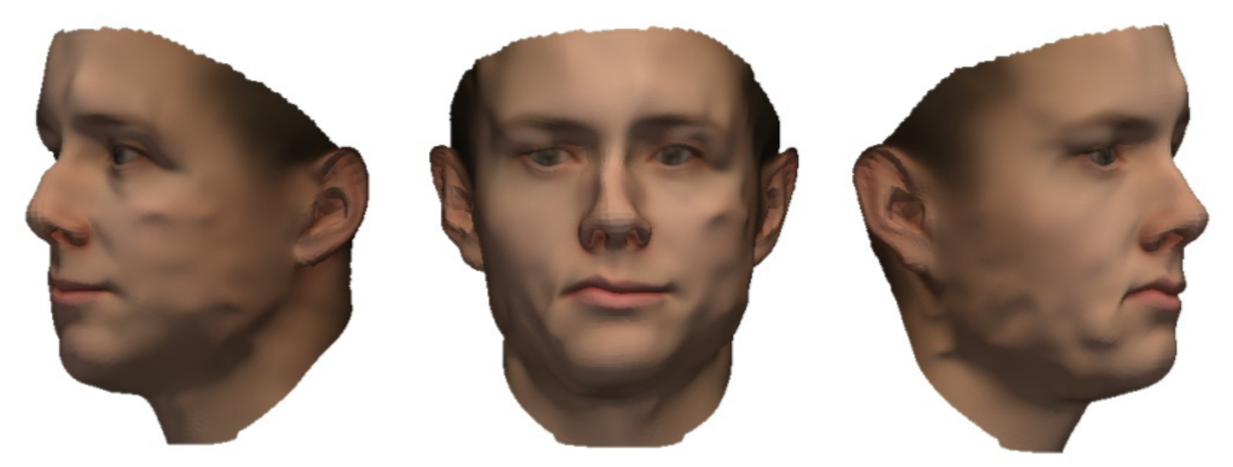
\includegraphics[width=.9\textwidth]{../resources/img/prior_sample_3_profile.pdf}
\end{figure}

\end{frame}
%%%%%%%%%%%%%%%%%%%%%%%%%%%%%%%%%%%%%%%%%%%%%%%%%%%%%%
\begin{frame}{Pipeline: Deformation Posterior}
\begin{figure}   
\centering
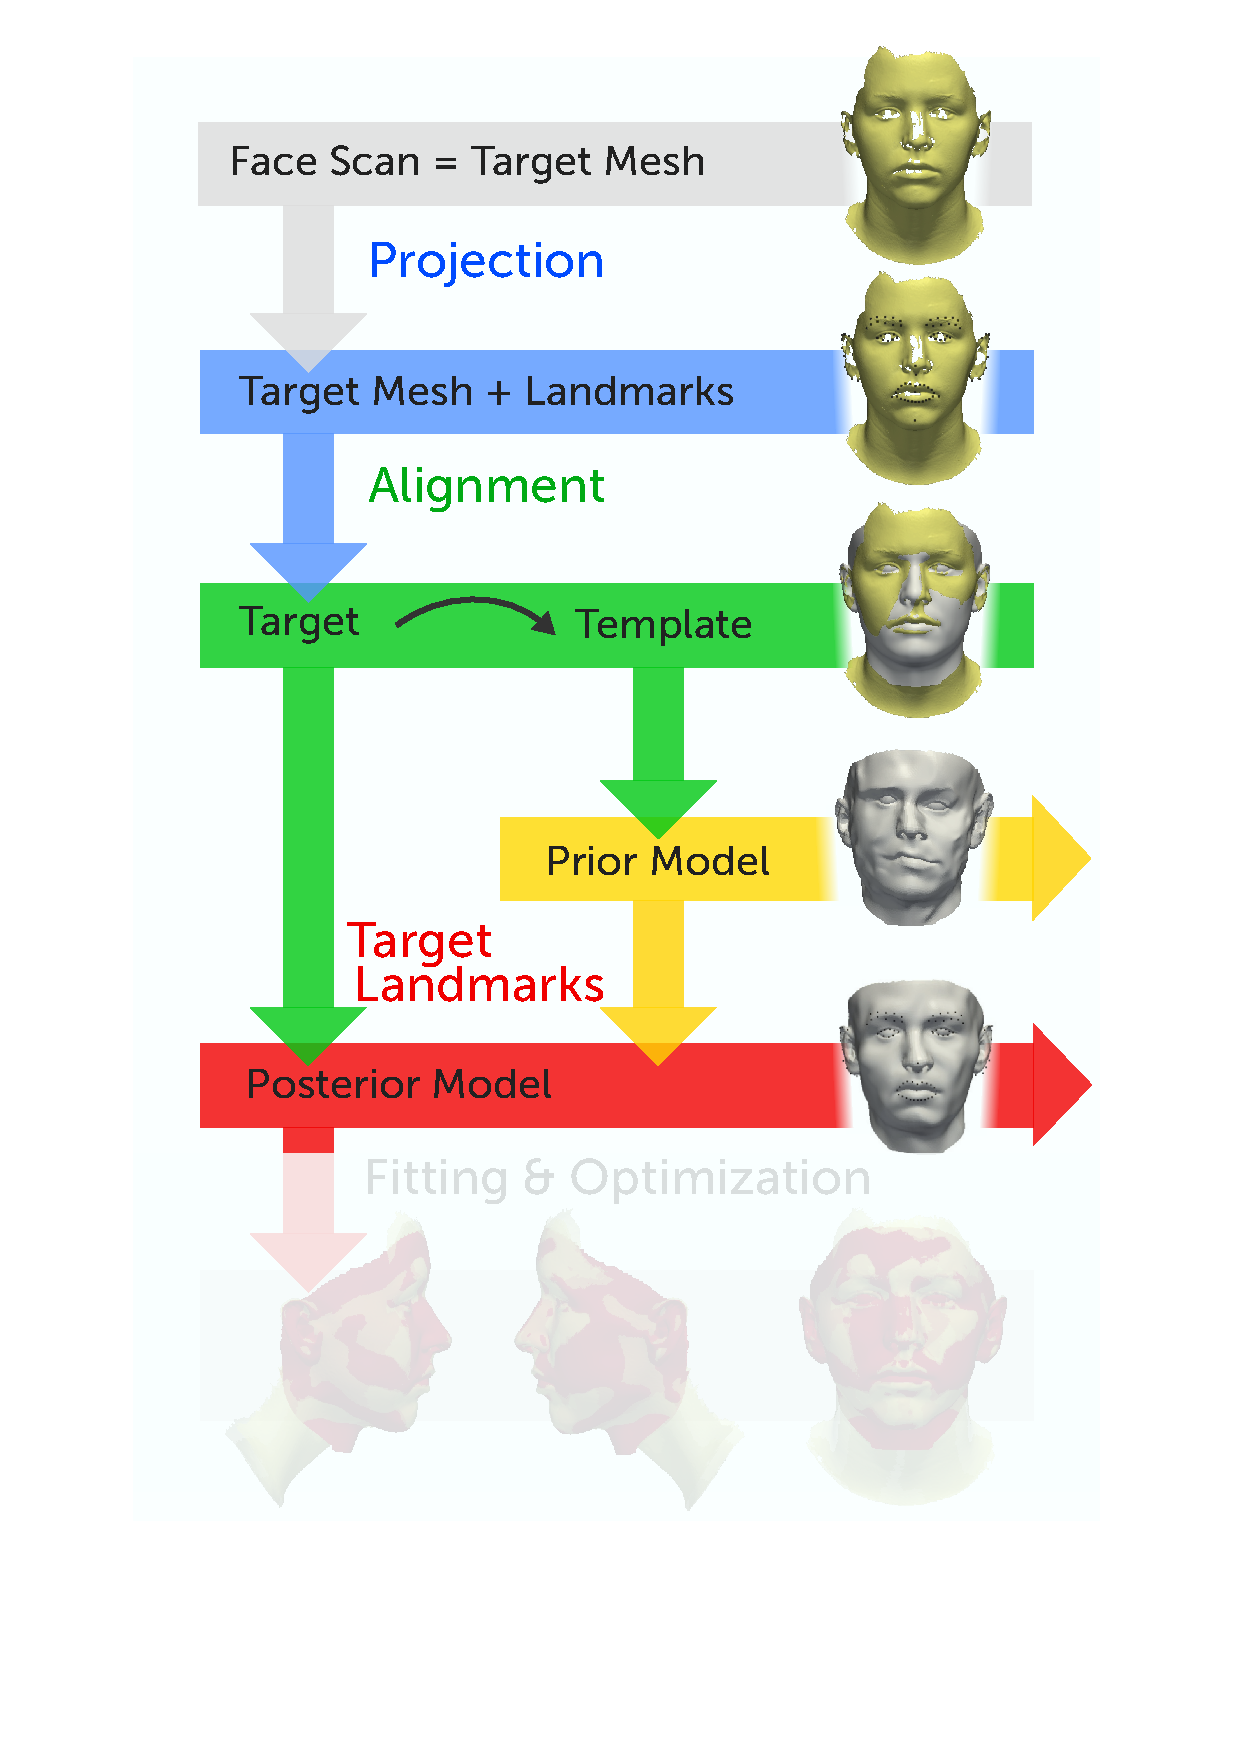
\includegraphics[width=.6\textwidth]{../resources/figures/pipeline_posterior.pdf}
\end{figure}
%\begin{comment}
%defined prior deformations on the template!
%now incorporate line features as additional landmarks.
%\end{comment}
\end{frame}

%%%%%%%%%%%%%%%%%%%%%%%%%%%%%%%%%%%%%%%%%%%%%%%%%%%%%%
\begin{frame}{3D GP Posterior}
inference in the space of possible template surface deformations\\
\bigskip
training data: residuals of the line feature sample coordinates:        
\begin{equation*}
R = \{t - m \vert t \in L_{T}, m \in L_{M}\} 
\end{equation*}
\begin{figure}   
\centering
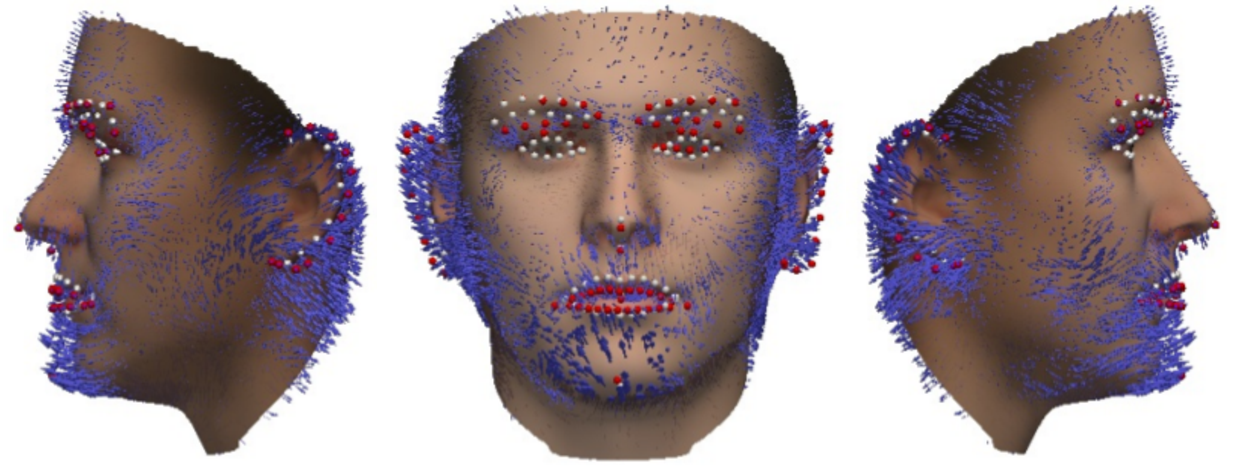
\includegraphics[width=.8\textwidth]{../resources/img/posterior_deformations.pdf}
\end{figure}

\end{frame}

\begin{frame}{Posterior Faces}
    \begin{figure}
        \centering
        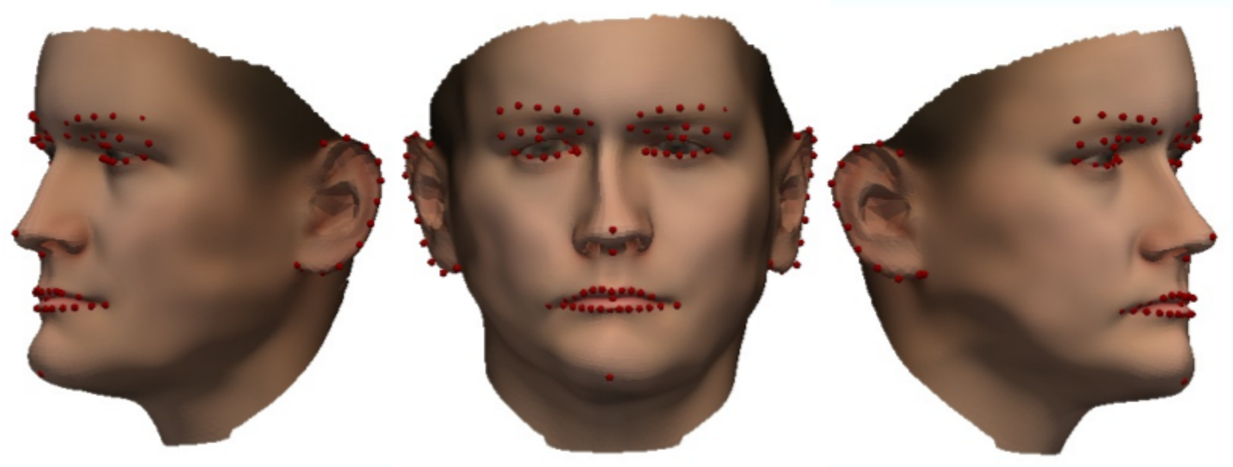
\includegraphics[width=.9\textwidth]{../resources/img/posterior_sample_17.pdf}
    \end{figure}
    \begin{figure}
        \centering
        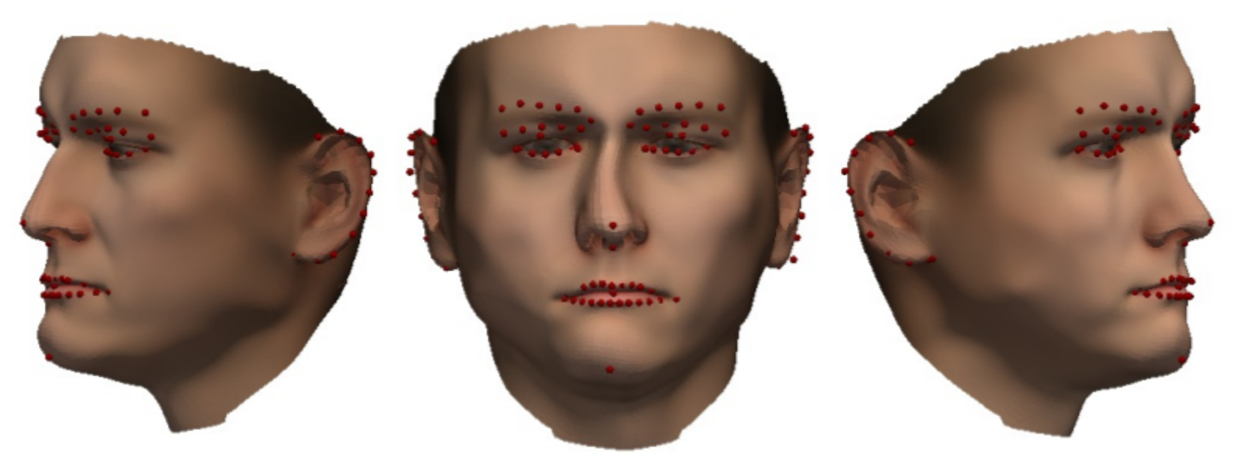
\includegraphics[width=.9\textwidth]{../resources/img/posterior_sample_23.pdf}
    \end{figure}
\end{frame}

\subsection{Optimization}
\begin{frame}{Fitting \& Optimization}
\begin{figure}
    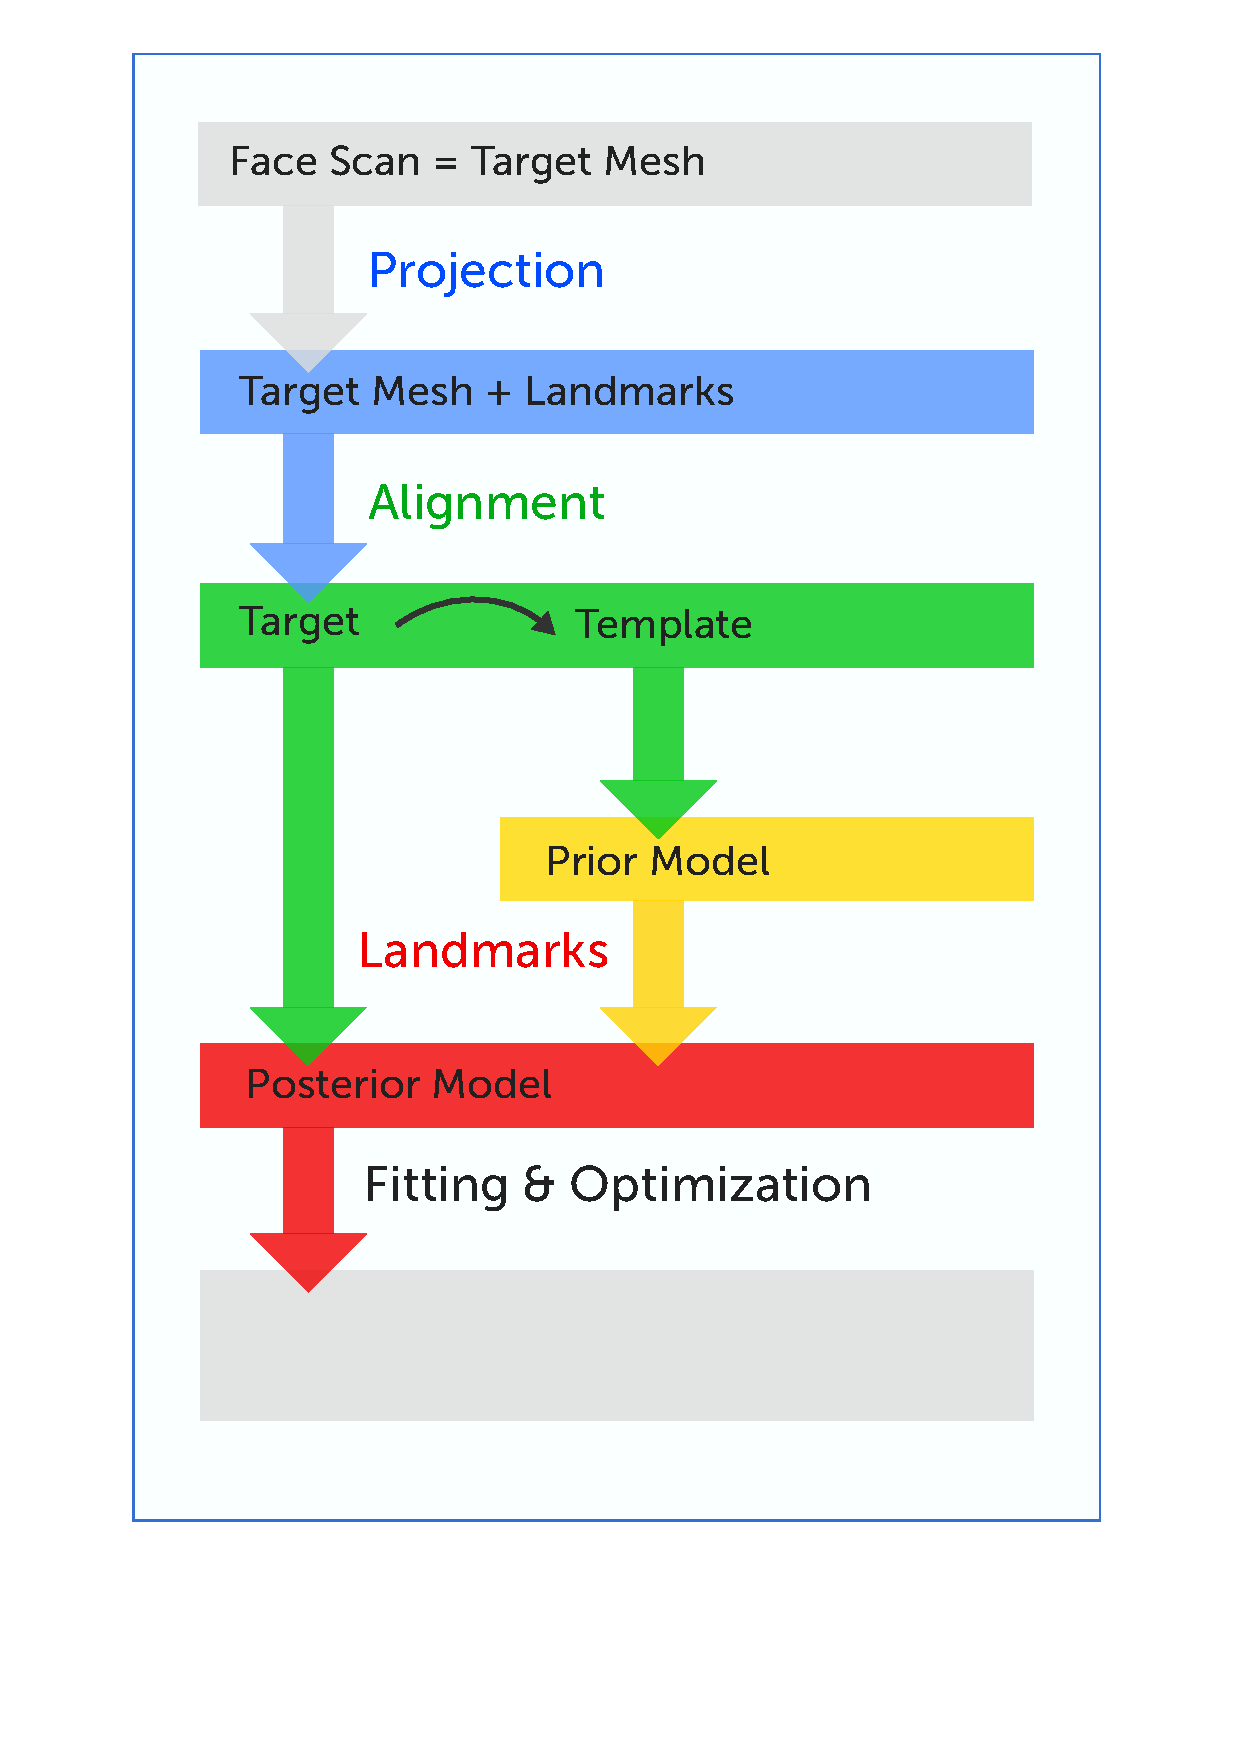
\includegraphics[width=.5\textwidth]{../resources/figures/pipeline.pdf}
\end{figure}
\end{frame}
\begin{frame}{Parametric Model}
    GP Posterior distribution of admissible deformations\\
    \bigskip
    How to optimize deformation samples?\\
    \bigskip
    Mercer's theorem: distribution $\rightarrow$ parametric model\\
    \bigskip
    $\Rightarrow$ optimize model parameters\\ verify with loss function
\end{frame}

\begin{frame}{Mean Squared Error}
    \begin{figure}
        \centering
        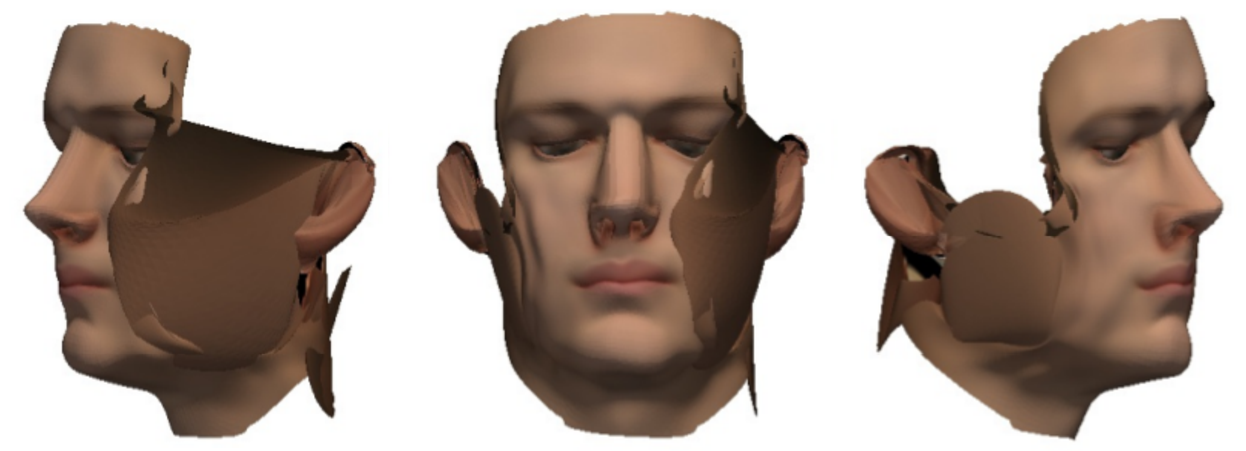
\includegraphics[width=\textwidth]{../resources/img/00029_meansquares_fit.pdf}
    \end{figure}
\end{frame}

\begin{frame}{Robust Estimator}
    \begin{figure}
        \centering
        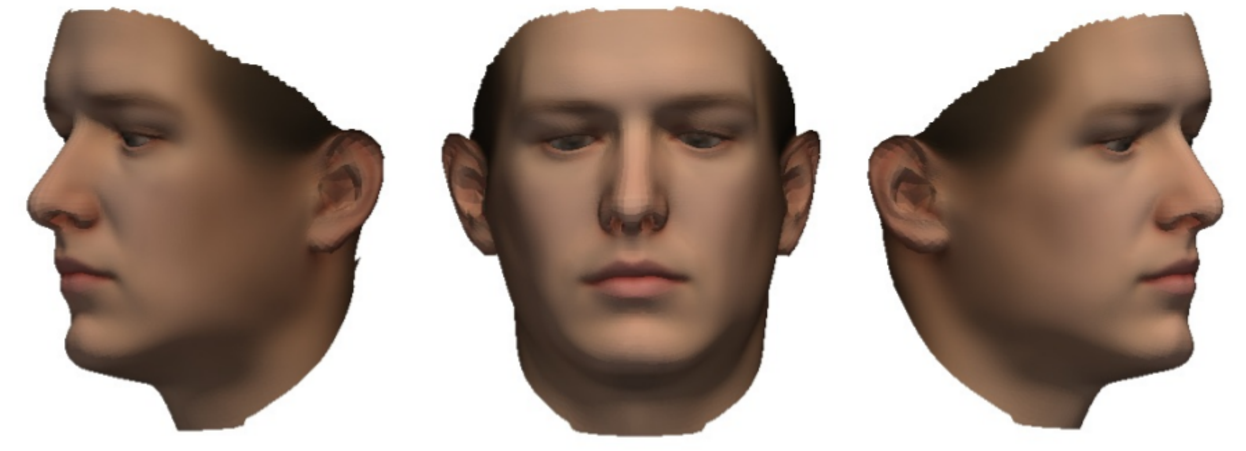
\includegraphics[width=.8\textwidth]{../resources/img/00029_fit.pdf}
    \end{figure}
    \begin{figure}
        \centering
        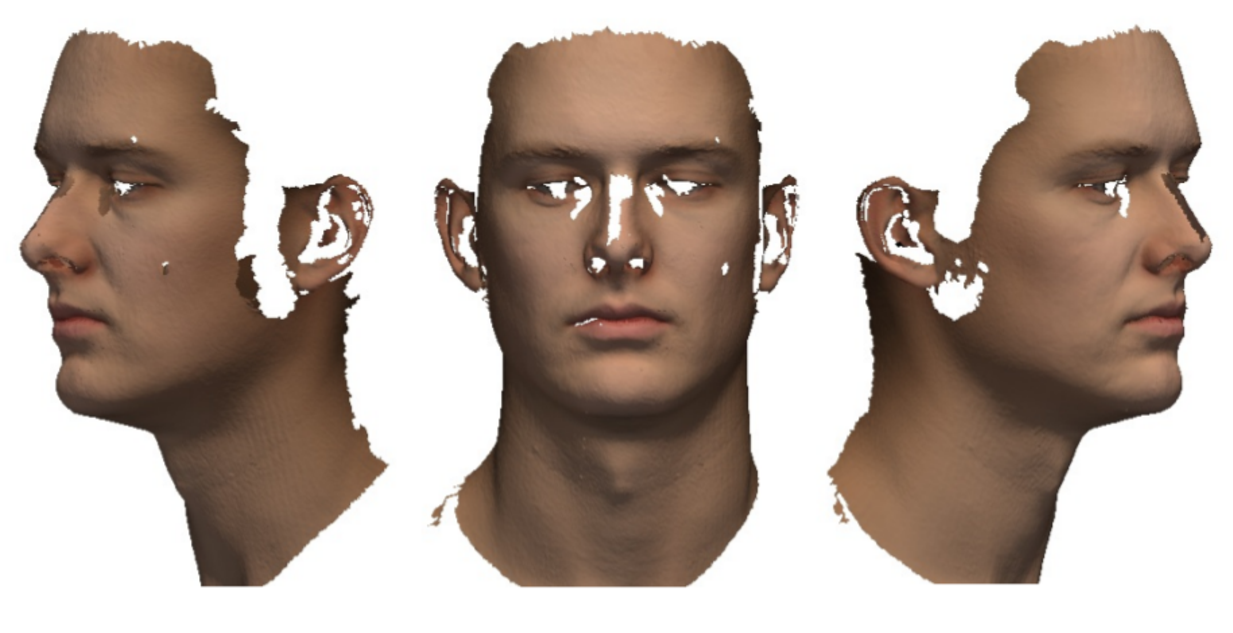
\includegraphics[width=.8\textwidth]{../resources/img/00029_textured_target.pdf}
    \end{figure}
\end{frame}

\begin{frame}{Robust Estimator}
    \begin{figure}
        \centering
        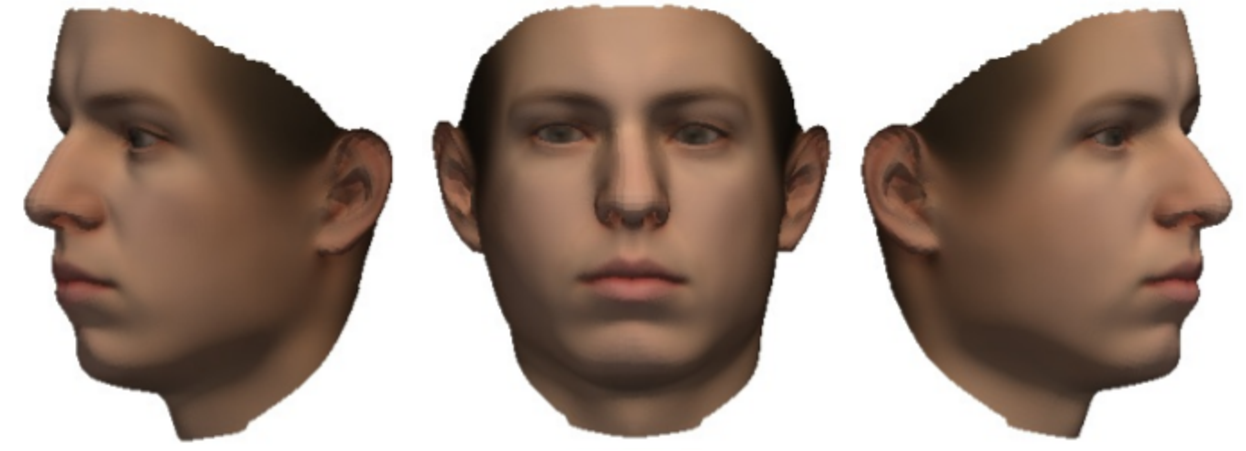
\includegraphics[width=.8\textwidth]{../resources/img/00303_fit.pdf}
    \end{figure}
    \begin{figure}
        \centering
        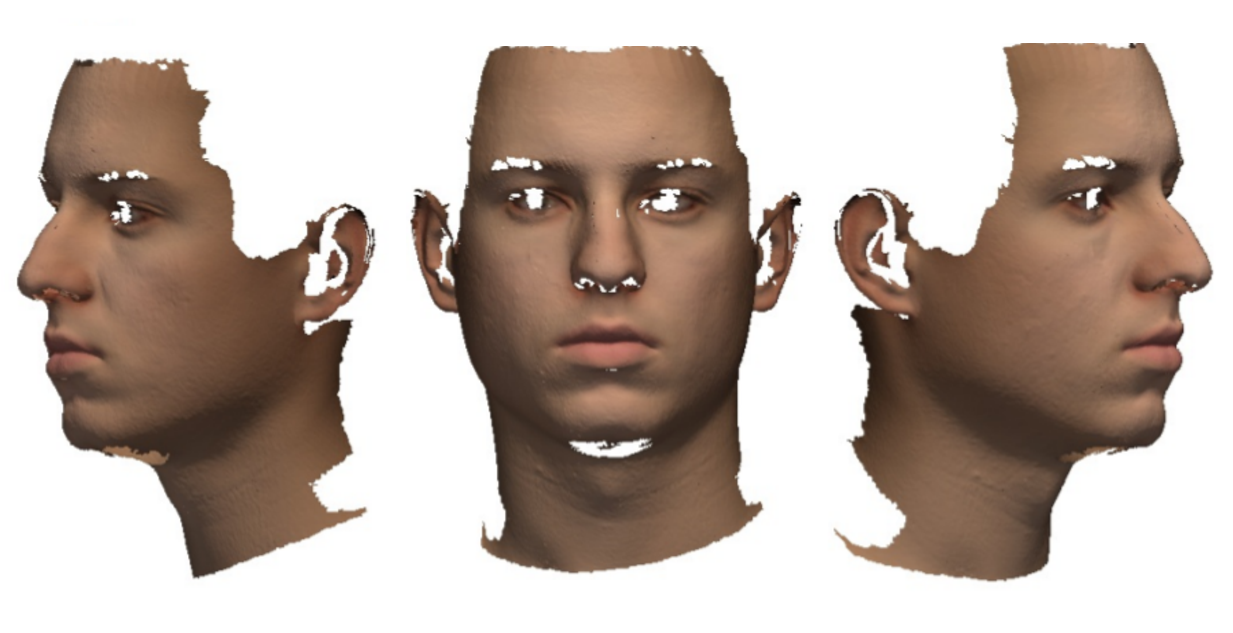
\includegraphics[width=.8\textwidth]{../resources/img/00303_textured_target.pdf}
    \end{figure}
\end{frame}

\begin{frame}{Pipeline: check}
\begin{figure}
    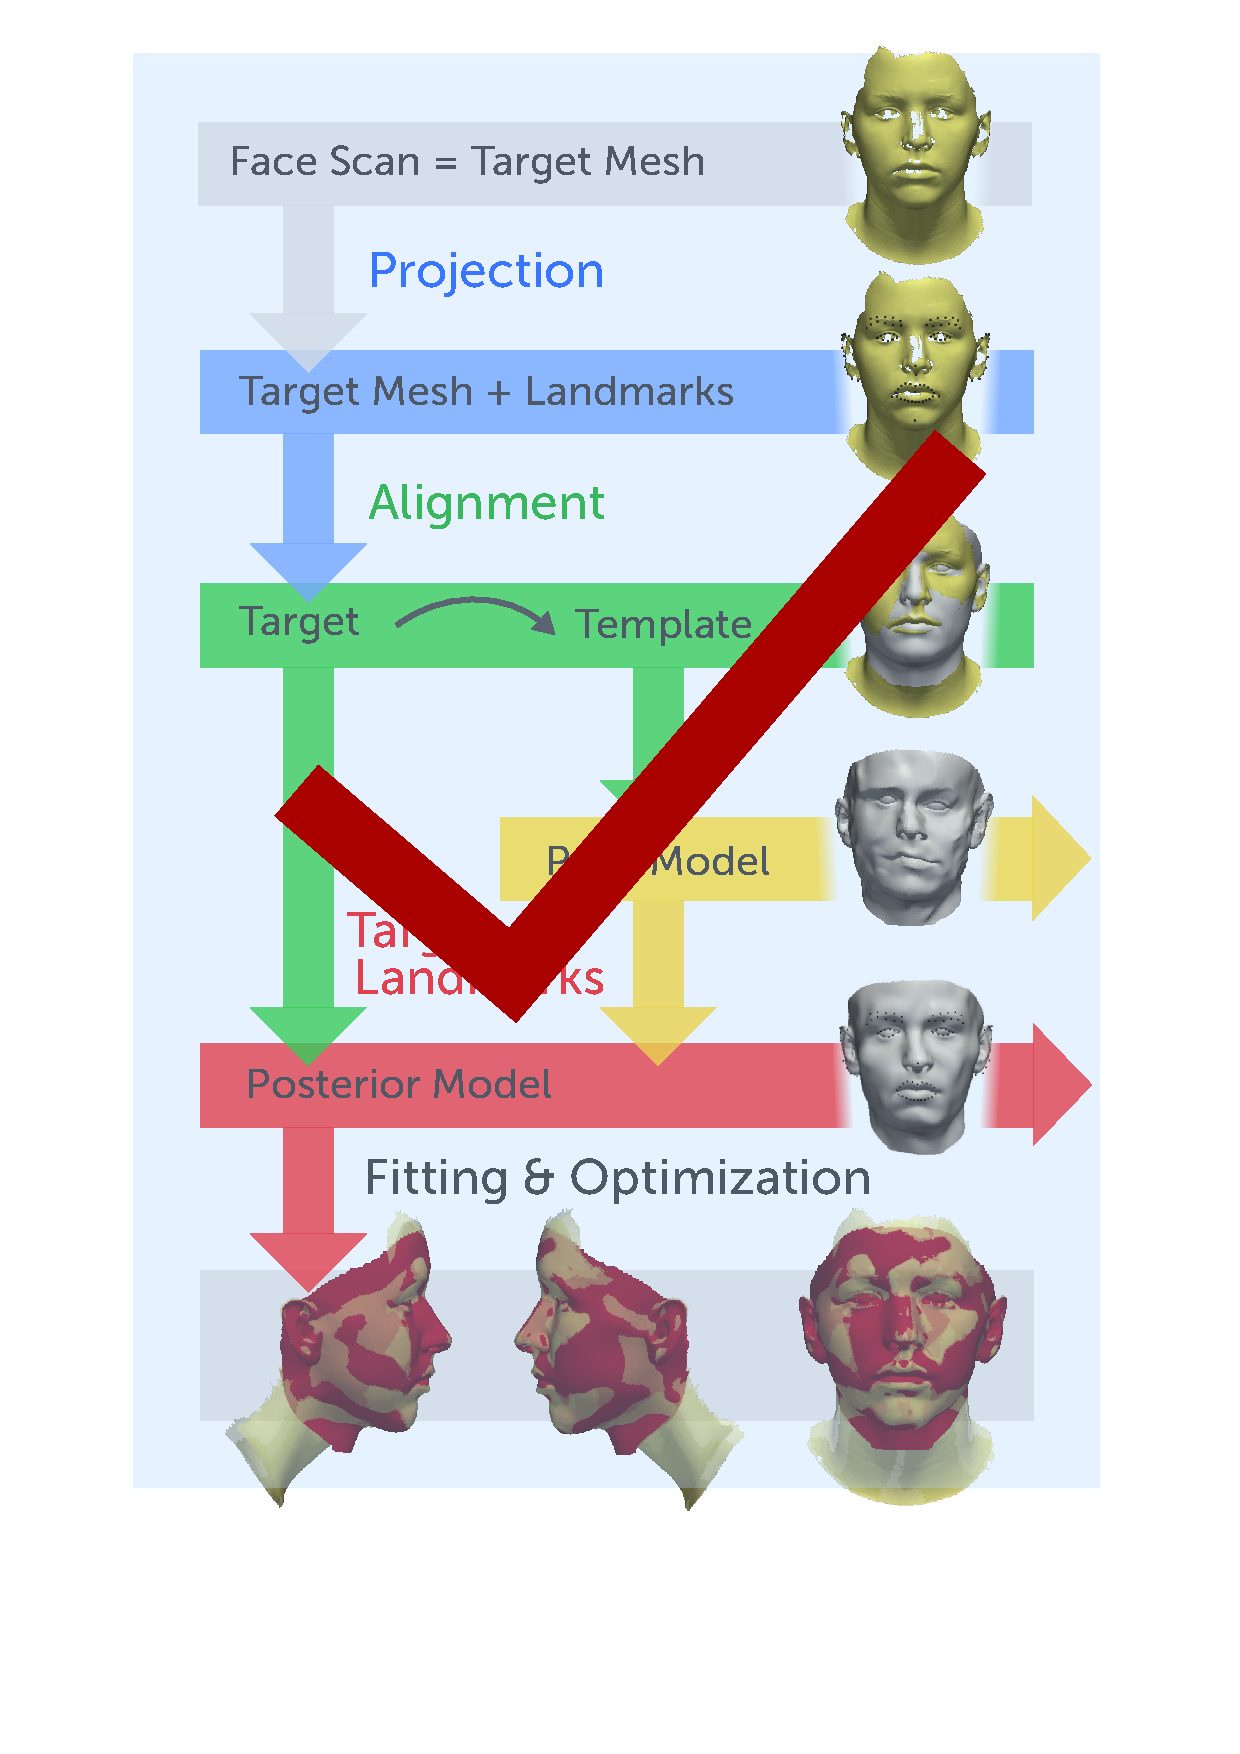
\includegraphics[width=.5\textwidth]{../resources/figures/pipeline_checked.pdf}
\end{figure}
\end{frame}

\section{Results}
\begin{frame}{Results}
\begin{itemize}
    \item    {\scshape Comparison: with $\Leftrightarrow$ without line features}
    \vfill
\item {\scshape Caricatures}
\end{itemize}
\end{frame}

\begin{frame}{Comparison - Mouth}
    \begin{figure}
        \centering
        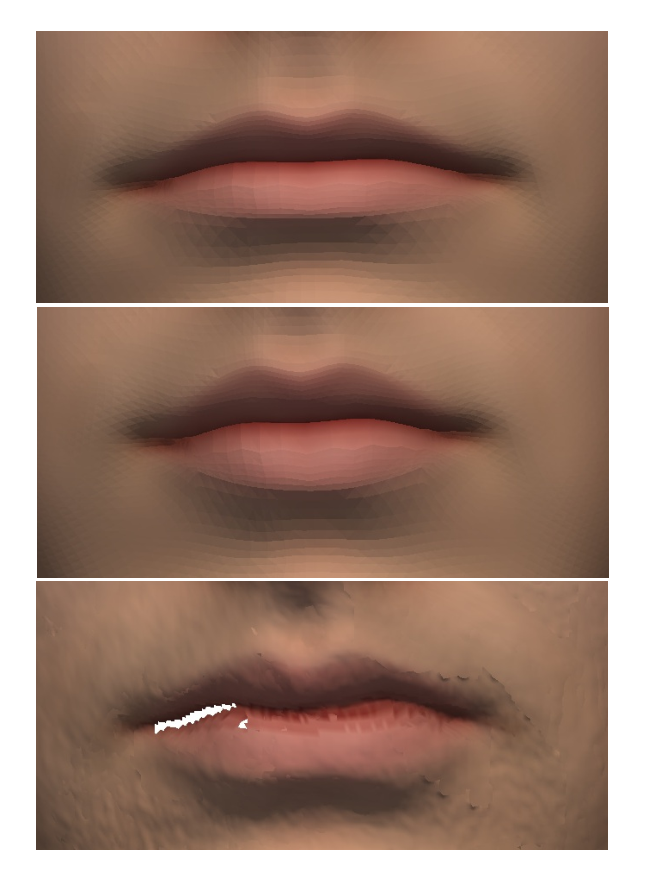
\includegraphics[width=.5\textwidth]{../resources/img/00029_mouth_comparison.pdf}
    \end{figure}
\end{frame}
\begin{frame}{Comparison - Eyes}
    \begin{figure}
        \centering
        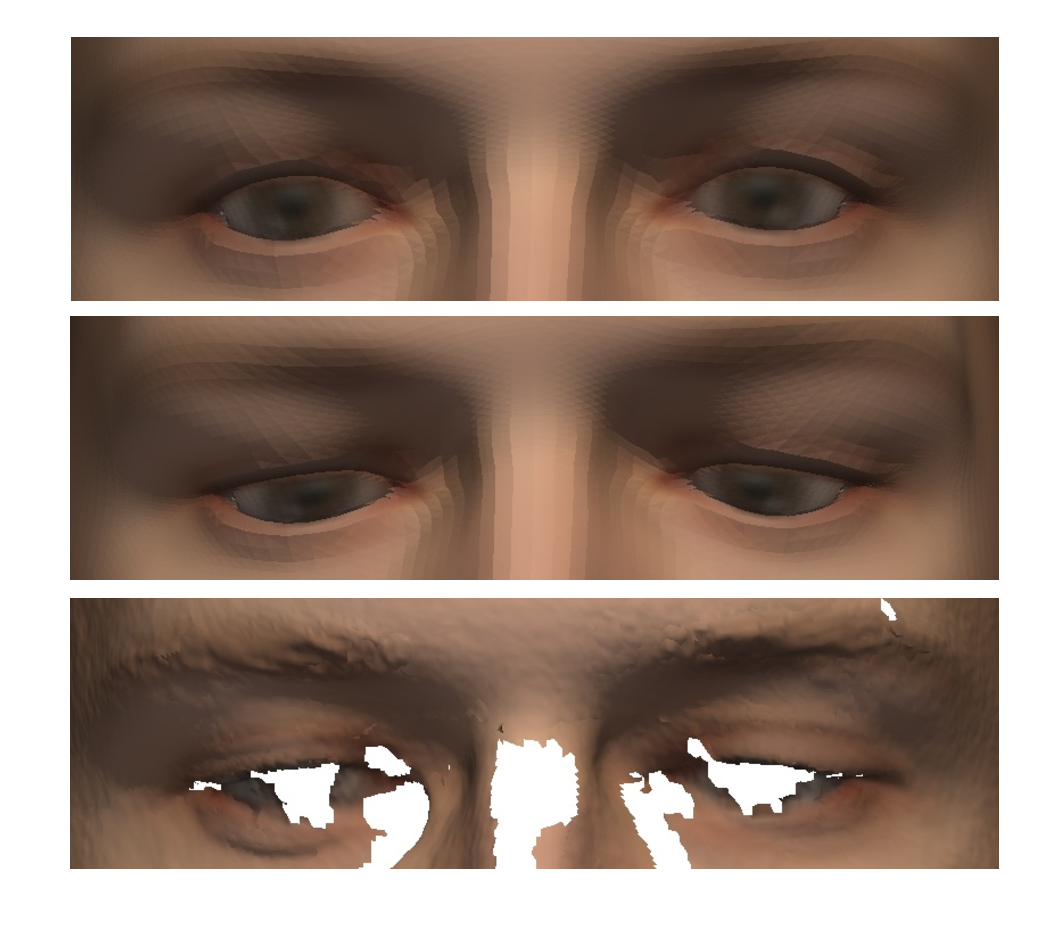
\includegraphics[width=.8\textwidth]{../resources/img/00029_eyes_comparison.pdf}
    \end{figure}
\end{frame}

\begin{frame}{Comparison - Ears}
    \begin{figure}
        \centering
        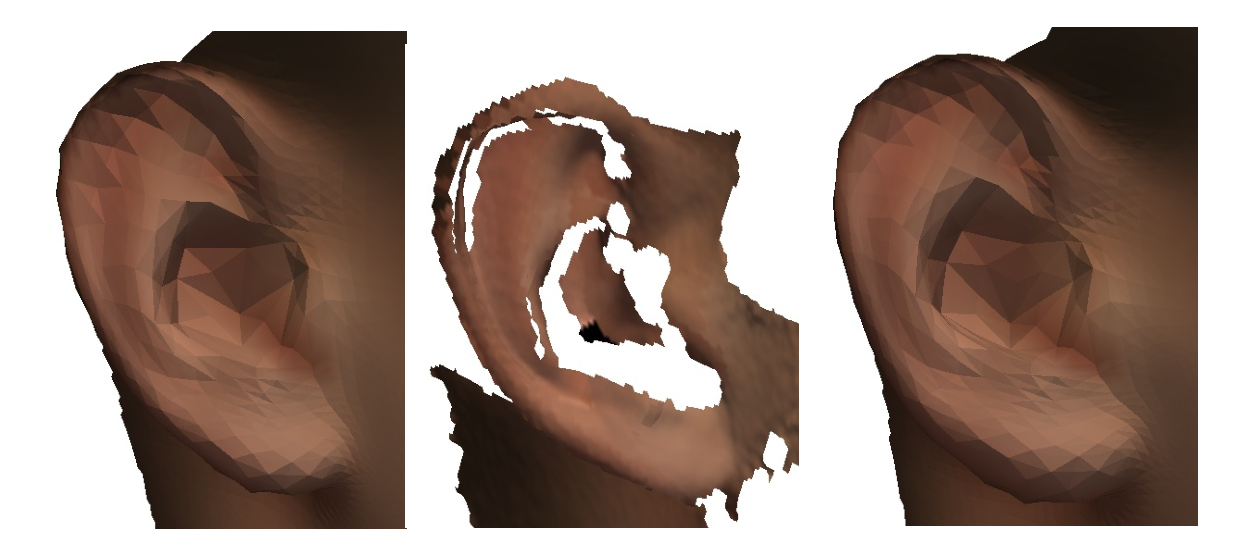
\includegraphics[width=.8\textwidth]{../resources/img/00029_left_ear_comparison.pdf}
    \end{figure}
\end{frame}

\begin{frame}{Caricatures}
    \movie[width=6cm, height=6cm, autostart]{hi}{00029_warp_animation.avi}
\end{frame}

\begin{frame}{Expressiveness}
    \begin{figure}
        \centering
        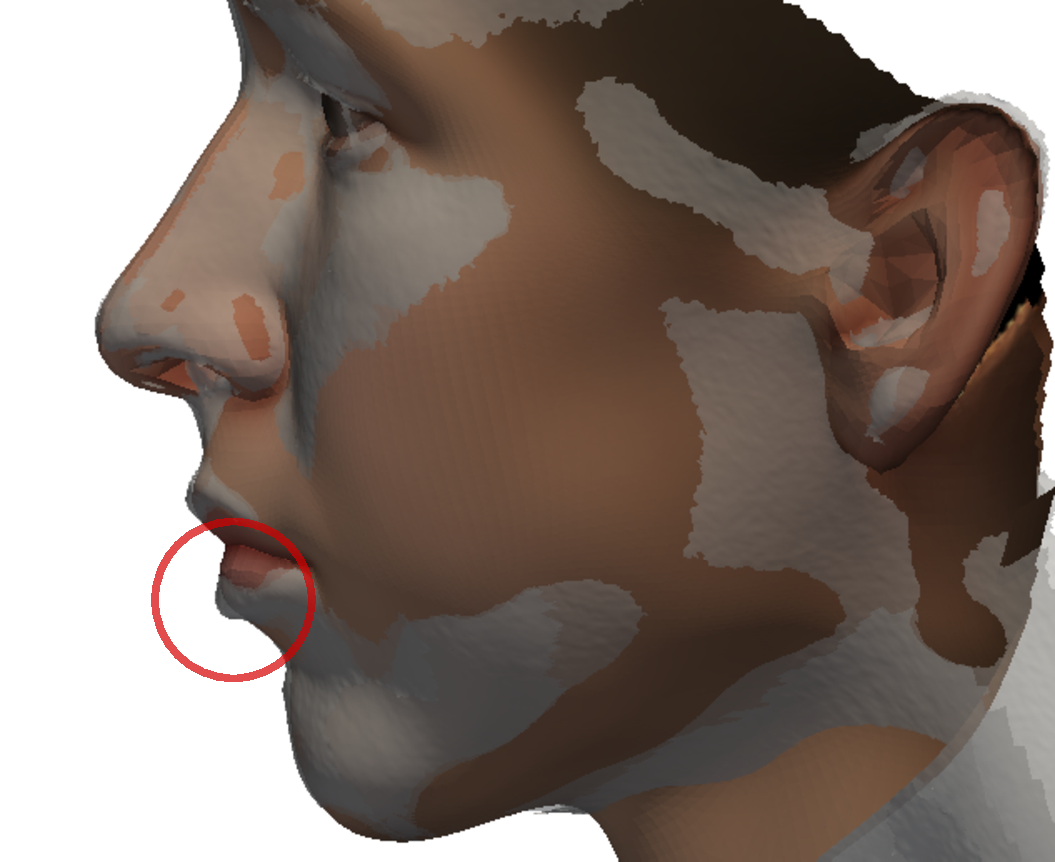
\includegraphics[width=.8\textwidth]{../resources/img/00041_expressiveness.pdf}
    \end{figure}
\end{frame}
\begin{frame}{Conclusion}
\begin{itemize}
\item Incorporation of line features rendered good registration results\\
\vfill  
\item Optimization process has to be further adapted for more expressiveness\\
\end{itemize}
\end{frame}

\begin{frame}{Future Work}
    detect template regions corresponding to \textbf{holes} in target\\
    detect template regions \textbf{missing} in target\\
    \bigskip
    by registering target on to template\\
    \vfill
    $\Rightarrow$ use Mean Squared Error to perform optimization without artifacts
\end{frame}
\begin{frame}{Thank you for listening!}
    \begin{center}
    \Large Any questions? 
    \end{center}
\end{frame}
\end{document}
